\documentclass[a4paper,12pt]{article}
\usepackage[serbian]{babel}
\usepackage{graphicx}
\usepackage{amsmath}
\usepackage{wrapfig}
\usepackage{embedfile}
\usepackage{microtype}
\usepackage{subcaption}
\usepackage[unicode]{hyperref}
\hypersetup{colorlinks, citecolor=blue, filecolor=blue, linkcolor=blue, urlcolor=blue}


\begin{document}

\begin{titlepage}
    \centering
    
    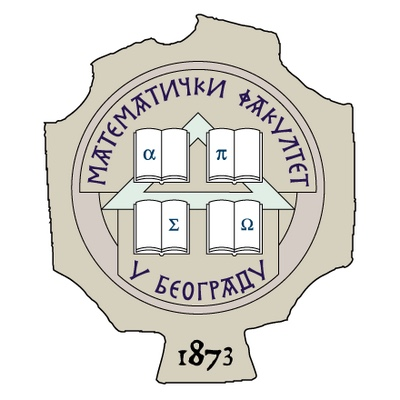
\includegraphics[width=0.3\textwidth]{matematickiFakultet.jpeg}\par
    
    Univerzitet u Beogradu\\ Matematički fakultet
    
    \vspace{2cm}
    
    \textbf{\Large ISTRAŽIVANJE UTICAJA P-ADIČNOSTI NA GENETSKI KOD KORONAVIRUSA: \\ \vspace{0.5cm} ANALIZA SEKVENCI I KLASTEROVANJE}
    
    \vspace{0.5cm}
    
    \ Seminarski rad iz predmeta Istraživanje podataka 2
    
    \vfill
    
    \begin{tabbing}
        \hspace{8cm} \= \kill
        \large \textbf{Profesor:} \> \large \textbf{Studenti:} \\
        \large Nenad Mitić \> \large Jelisaveta Gavrilović 188/2020 \\
        \> \large Marko Paunović 104/2020
    \end{tabbing}
    
    \vspace{0.5cm}
    \large Beograd, maj 2024.
    
\end{titlepage}
\newpage

\tableofcontents
\newpage

\section{Uvod}
Genetski kod predstavlja osnovu biološke informacije u svim živim organizmima. On je ključan za 
razumevanje procesa genetičke ekspresije i sinteze proteina, te ima glavnu ulogu u 
prenošenju genetičke informacije. 

\medskip
Koronavirusi su velika porodica virusa koji mogu izazvati bolesti kod životinja i ljudi. Kod ljudi, poznato je da nekoliko koronavirusa izaziva respiratorne infekcije koje mogu varirati od blagih prehlada do ozbiljnijih bolesti kao što su Middle East Respiratory Syndrome Coronavirus (MERS), Severe Acute Respiratory Syndrome Coronavirus (SARS) i COVID-19, bolest uzrokovana novim koronavirusom SARS-CoV-2. Zbog brzine širenja i potencijalno teških posledica po zdravlje, istraživanje genetske strukture koronavirusa je od presudnog značaja za razvoj dijagnostičkih alata, terapija i vakcina.

\bigskip
Mi ćemo se fokusirati na analizu genetskog koda nekoliko značajnih koronavirusa: SARS-CoV 
(uzročnik SARS-a), MERS-CoV (uzročnik MERS-a), Bovine coronavirus (BCoV), Human 
coronavirus 229E (HCoV-229E) i Human coronavirus OC43 (HCoV-OC43). Ovi virusi 
predstavljaju različite grupe koronavirusa sa značajnim genetskim i epidemiološkim 
karakteristikama.

\medskip
Cilj ovog rada je analizirati uticaj p-adičnosti na razlike u genetskom kodu između ovih različitih vrsta koronavirusa. P-adična analiza pruža novi pristup proučavanju genetskog koda, Kombinacija p-adičnih rastojanja i Hammingovih rastojanja omogućava detaljno poređenje genetskih sekvenci na 
molekularnom nivou, što može pružiti uvid u evolutivne procese i funkcionalne razlike.

\medskip
Osim toga, istraživanje će se fokusirati i na upotrebu hijerarhijskog klasterovanja za grupisanje 
genetskih sekvenci na osnovu njihovog edit rastojanja. Ovakav pristup omogućava otkrivanje grupa sličnih 
sekvenci koje mogu ukazati na zajedničko poreklo ili funkcionalnu povezanost.

\bigskip
U implementaciji i analizi, koristićemo sledeće biblioteke: Biopython za rad sa biološkim podacima \cite{cock2009biopython}, scikit-learn za primenu hijerarhijskog klasterovanja i PCA \cite{pedregosa2011scikit}, NumPy za numeričke proračune \cite{harris2020array}, pandas za obradu i analizu podataka \cite{mckinney2010data}, matplotlib za kreiranje grafikona \cite{hunter2007matplotlib} i seaborn za unapređene statističke vizualizacije \cite{waskom2020seaborn}.

Potrebne biblioteke možete instalirati pokretanjem sledeće komande iz terminala:
\small
\begin{verbatim}
pip install biopython scikit-learn numpy pandas matplotlib seaborn
\end{verbatim}
\normalsize

Ceo kod istraživanja dostupan je na GitHub platformi \cite{github_link1, github_link2}.


\newpage
\section{Genetski kod}
Sveukupna genetska informacija jednog organizma naziva se genom, a sva genetska informacija nalazi se u molekulu DNK. Svaki funkcionalni region molekula DNK naziva se gen. Gen je fizička i funkcionalna jedinica nasleđivanja koja prenosi naslednu poruku iz generacije u generaciju, a čini ga celovit deo DNK potreban za sintezu jednog proteina ili jednog molekula RNK. Svaki gen se putem procesa transkripcije prevodi u odgovarajući molekul RNK, koji se procesom translacije prevodi u sekvencu aminokiselina.

\begin{wrapfigure}{r}{0.4\textwidth}
    \hspace{-1.1cm}
    \vspace{-0.3cm}
  \centering
  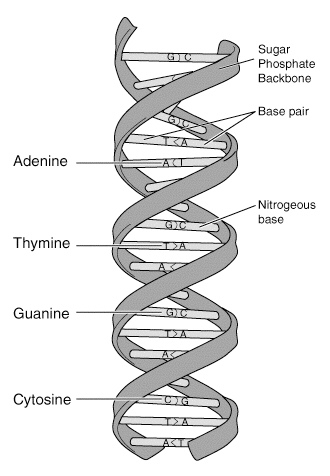
\includegraphics[width=0.48\textwidth]{slika1.jpeg}
  \caption{DNK molekul}
\end{wrapfigure}

\bigskip
Genetski kod je jezik za prenošenje genetske poruke od DNK (gena) do proteina i sadržan je u redosledu baza na lancu DNK. Celokupan genetski kod sastoji se od jedinstvenog kombinovanja četiri tipa nukleotida DNK. Svaki nukleotid se sastoji od podgrupe koju čine fosfatna grupa, šećer dezoksiriboze i jedna od četiri moguće azotne baze, koje su grupisane u dve kategorije: purini i pirimidini. Purinske baze Adenin (A) i Guanin (G) su veće i sastoje se od dva aromatična prstena. Pirimidinske baze Citozin (C) i Timin (T) su manje i sastoje se od jednog aromatičnog prstena. Jedinica genetskog koda je niz od tri nukleotida (triplet) DNK i on se u celini komplementarno prenosi, transkripcijom, na informacionu RNK. Kod molekula RNK, Timin je zamenjen Uracilom (U) i šećer dezoksiriboze je zamenjen šećerom riboze. Triplet na informacionoj RNK naziva se \textbf{kodon} i predstavlja šifru za jednu aminokiselinu, dok niz kodona šifruje polipeptidni lanac.

\bigskip
Početak translacije zahteva prisustvo male ribozomalne jedinice koja se vezuje za start kodon na i-RNK, što zauzvrat označava gde i-RNK počinje da kodira određeni protein. U 98\% slučajeva ovaj kodon je AUG. Proces elongacije traje sve dok ribozom ne naiđe na jedan od tri moguća stop kodona: UAA, UAG ili UGA, kada se translacija završava. Tada se zaustavlja sinteza polipeptidnog lanca i protein se oslobađa u citoplazmu.

\newpage
\begin{figure}[h!]
  \centering
  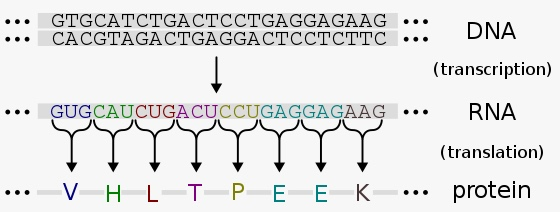
\includegraphics[width=0.8\textwidth]{slika2.jpeg}
  \caption{Proces prevođenja sekvence DNK molekula u protein}
  \label{fig:my_label}
\end{figure}

\bigskip
Genetski kod je eksperimentalno otkriven sredinom 1960-ih \cite{bernfield1965}, što nam omogućava da razumemo kako funkcioniše u praksi, ali njegovo teorijsko razumevanje i dalje nije potpuno. Skoro sve žive vrste koriste isti genetski kod, poznat kao standardni genetski kod, dok samo mali broj organizama pokazuje male varijacije u ovom kodu.


\begin{figure}[h!]
  \centering
  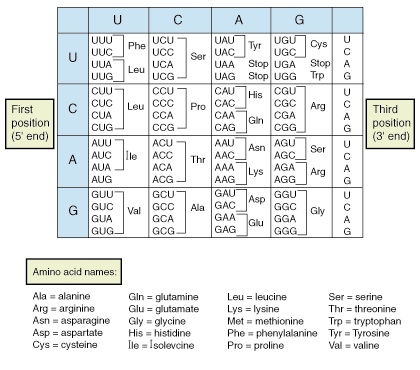
\includegraphics[width=0.8\textwidth]{slika3.jpeg}
  \caption{Standardni genetski kod}
  \label{fig:my_label}
\end{figure}

\section{Preprocesiranje podataka}
Nakon što smo se upoznali sa osnovama genetskog koda i procesima transkripcije i translacije, preprocesiranje referentnih genoma i proteina predstavlja naredni korak za pripremu podataka za detaljnu analizu. Svi podaci su preuzeti iz javno dostupne baze podataka Nacionalnog Centra za Biotehnološke Informacije (NCBI) \cite{ncbi_database}.

\bigskip
Jedan od najvažnijih koraka preprocesiranja je identifikacija otvorenih okvira za čitanje (ORF-ova).
ORF-ovi su nizovi nukleotida u RNK koji potencijalno kodiraju proteine. Pronalaženjem ORF-ova,
identifikovali smo regione koji mogu biti prepisani i prevedeni u proteinske sekvence.

\medskip
Zašto je ovo važno? 

\smallskip
Kodiranje proteina započinje identifikacijom odgovarajućih sekvenci u RNK koje sadrže informaciju o proteinskoj strukturi. Međutim, prema standardnom genetskom kodu jedna aminokiselina može biti kodirana različitim kombinacijama kodona. To znači da istu proteinsku sekvencu možemo prevesti iz više različitih RNK sekvenci. Identifikacija ORF-ova omogućila nam je precizno mapiranje ovih kodirajućih delova RNK, što nam je pomoglo u određivanju pozicija potencijalno kodirajućih delova RNK.

\begin{figure}[h!]
  \centering
  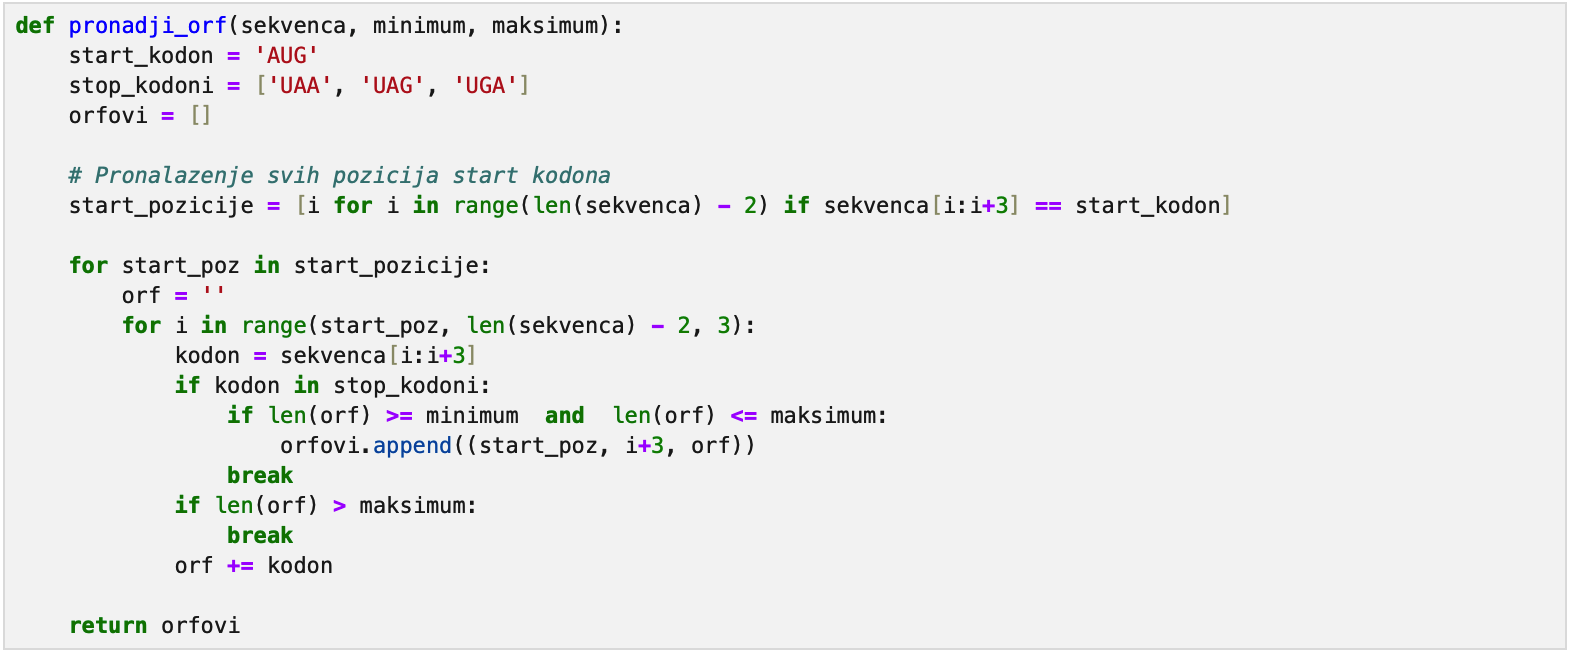
\includegraphics[width=1\textwidth]{slika4.jpeg}
  \caption{Funkcija za pronalaženje ORF-ova}
  \label{fig:my_label}
\end{figure}

Nakon identifikacije ORF-ova, možemo prevesti RNK sekvence u sekvence aminokiselina  koristeći standardni genetski kod. Zatim upoređujemo dobijene proteinske sekvence sa referentnim proteinskim sekvencama kako bismo identifikovali koje sekvence kodiraju poznate proteine.

\newpage

\begin{figure}[h!]
  \centering
  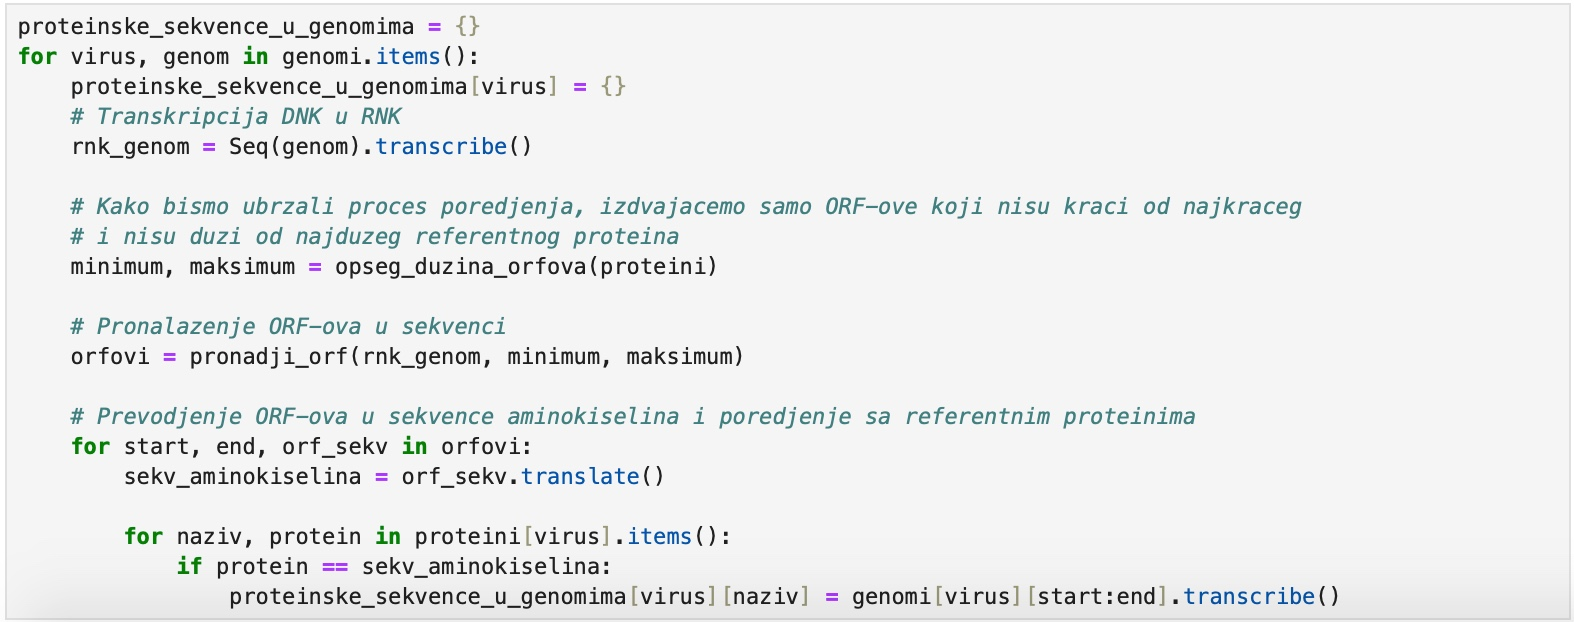
\includegraphics[width=1\textwidth]{slika5.jpeg}
  \caption{Poređenje dobijenih proteinskih sekvenci sa referentnim proteinima}
  \label{fig:my_label}
\end{figure}

\bigskip
Iako smo uspeli da identifikujemo većinu proteina ovom metodom, neki proteini nisu mogli biti automatski pronađeni. Za te proteine koristili smo dodatne informacije iz NCBI baze podataka kako bismo ručno odredili njihove pozicije u genomima. Ova ručna dopuna osigurava da imamo kompletan skup proteinskih sekvenci za dalju analizu.

\begin{figure}[h!]
  \centering
  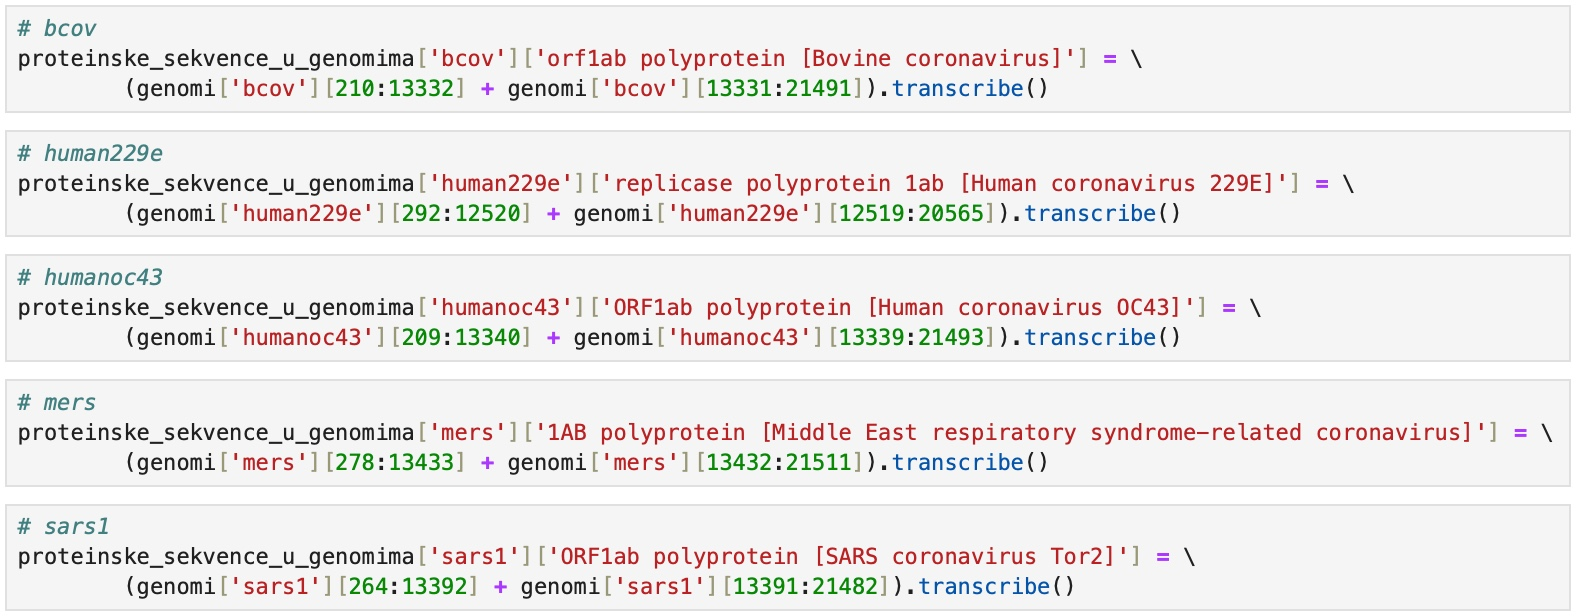
\includegraphics[width=1\textwidth]{slika6.jpeg}
  \caption{Ručno dodati proteini}
  \label{fig:my_label}
\end{figure}

\bigskip
Ceo kod korišćen za preprocesiranje podataka možete pogledati u datoteci 
\texttt{preprocesiranje.ipynb}. Rezultati koji su dobijeni su smešteni u datoteci \texttt{rnk.fasta} koja se nalazi u direktorijumu \texttt{proteini}, poddirektorijumu \texttt{podaci}.

\newpage
\section{Analiza površinskih proteina}
Površinski proteini koronavirusa, posebno spike (S) proteini, igraju ključnu ulogu u inficiranju domaćina. Oni omogućavaju virusu da se veže za receptore na ćelijama domaćina, što je prvi korak u procesu ulaska virusa u ćeliju. Razlike u ovim proteinima među različitim vrstama koronavirusa rezultiraju različitim receptorima na koje se virus vezuje, što utiče na patogenezu i prenosivost virusa.

\bigskip
Na primer, spike protein SARS-CoV-1 virusa se vezuje za ACE2 receptor na ćelijama domaćina. ACE2 receptor se široko nalazi na površini ljudskih ćelija, posebno u respiratornom traktu, što objašnjava visoku stopu infektivnosti ovog virusa. Sa druge strane, MERS-CoV koristi DPP4 receptor za ulazak u ćelije domaćina, što rezultira drugačijom patogenezom i manjom stopom prenosa u poređenju sa SARS-CoV-1.
Spike protein HCoV-229E virusa se vezuje za APN receptor na ćelijama domaćina. Ova specifičnost omogućava HCoV-229E da efikasno inficira ljude, ali obično izaziva blaže respiratorne infekcije. 

\smallskip
Pored spike proteina, neki koronavirusi, poput BCoV i HCoV-OC43, koriste hemaglutinin-esterazu (HE) protein za ulazak u ćelije domaćina. Ova specifičnost omogućava BCoV-u da inficira goveda, dok HCoV-OC43 inficira ljude.

\smallskip
\begin{figure}[h!]
  \centering
  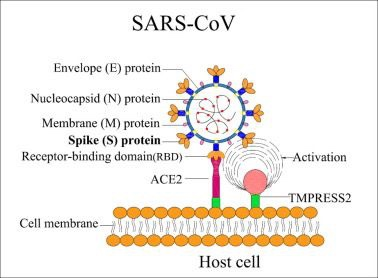
\includegraphics[width=0.64\textwidth]{slika7.jpeg}
  \caption{Vezivanje SARS-CoV za ćeliju domaćina}
  \label{fig:my_label}
\end{figure}

\bigskip
Korišćenjem p-adičnog i Hamingovog rastojanja, istražićemo razlike i sličnosti između ovih proteina na molekularnom nivou. Kod koji koristimo se nalazi u datoteci \texttt{povrsinski\_proteini\_rastojanja.ipynb}.


\newpage
\subsection{P-adično rastojanje}
P-adično rastojanje je ključni koncept u našoj analizi površinskih proteina i predstavlja matematički alat za modeliranje genetskog koda. Ovaj pristup, predložen 2006. godine od strane Dragovića i Dragovića \cite{dragovic2006}, istražuje bliskost kodona koji kodiraju istu aminokiselinu u ultrametričnom prostoru, uvodeći p-adični prostor kodona za p = 5 i p = 2. 

\bigskip
Sada ćemo ukratko objasniti šta su p-adični brojevi.

\smallskip
P-adični brojevi predstavljaju cele brojeve u specifičnom sistemu zasnovanom na prostom broju p. Ovaj pristup omogućava određivanje udaljenosti između brojeva korišćenjem p-adične norme, koju označavamo: \(\lvert x \rvert_{p}\).

Neka su x i y dva cela broja, 
\[ 
x = x_{0} + x_{1}p + x_{2}p^{2} + \ldots + x_{k}p^{k} \equiv x_{0}x_{1}x_{2}\ldots x_{k}
\],
\[ y = y_{0} + y_{1}p + y_{2}p^{2} + \ldots + y_{k}p^{k} \equiv y_{0}y_{1}y_{2}\ldots y_{k}
\]

\bigskip
gde su \( x_i \in \{0, 1, \ldots, p-1\} \) i \( y_i \in \{0, 1, \ldots, p-1\} \) cifre brojeva u odgovarajućoj \( p \)-adičnoj bazi, a \( \equiv \) je oznaka za drugačiji zapis broja x, odnosno y. Tada se udaljenost između x i y računa kao:

\[
d_{p}(x, y) = |x - y|_{p} = \begin{cases}
    1 & \text{, } x_{0} \neq y_{0} \\
    \frac{1}{p} & \text{, } x_{0} = y_{0} \text{, } x_{1} \neq y_{1} \\
    \frac{1}{p^2} & \text{, } x_{0} = y_{0} \text{, } x_{1} = y_{1} \text{, } x_{2} \neq y_{2} \\
    \vdots & \\
    \frac{1}{p^k} & \text{, } x_{0} = y_{0} \text{, } \ldots \text{, } x_{k-1} = y_{k-1} \text{, } x_{k} \neq y_{k}
\end{cases}
\]

\bigskip
U našem kontekstu, p-adični pristup omogućava analizu “bliskosti" između kodona koji kodiraju istu aminokiselinu u genetskom kodu. 

\medskip
Korišćenjem Dragovićevog modela koji se oslanja na 5-adično rastojanje, prvo su pridruženi odgovarajući brojevi kodonima. Ova konstrukcija brojeva temelji se na prirodnim karakteristikama nukleotida:

Kao što je ranije rečeno, postoje tri pirimidinske (C, T, U) i tri purinske (A, G, I) azotne baze, gde I označava inozin koji se može koristiti kao deo antikodona transportne RNK (tRNK) kako bi se omogućilo uparivanje sa više različitih kodona, što doprinosi fleksibilnosti i efikasnosti procesa translacije. Budući da su Timin (T) i Uracil (U) praktično ekvivalentni, ostaje pet nukleotida kojim treba pridružiti odgovarajućih pet cifara (jer p = 5) uzimajući u obzir da su purini (A, G) i pirimidini (C, U) međusobno sličniji nego purin u poređenju sa pirimidinom. Ova sličnost je prirodno opisana kroz 2-adično rastojanje. 

Pošto je inozin poseban slučaj njemu je dodeljen broj 0, to nas to dovodi do toga da je \(A \equiv 2\) i \(G \equiv 4\) ili \(G \equiv 2\) i \(A \equiv 4\) jer \(d_{2}(0, 2) = d_{2}(4, 2) = \frac{1}{2}\)
. Tada bi trebalo da bude \(C \equiv 1\) i \(U \equiv 3\) ili \(U \equiv 1\) i \(C \equiv 3\). Zbog uparivanja baza (A, U) i (C, D) trebalo bi da važi \(A + U = C + G = 5\). 

Na kraju, uzete su sledeće vrednosti za nukleotide: 

\[
I \equiv 0, C \equiv 1, A \equiv 2, U (T) \equiv 3, G \equiv 4.
\]

\bigskip
Na osnovu identifikacije nukleotida, kodonima iz standardnog genetskog koda dodeljeni su brojevi:

\bigskip
\begin{figure}[h!]
  \centering
  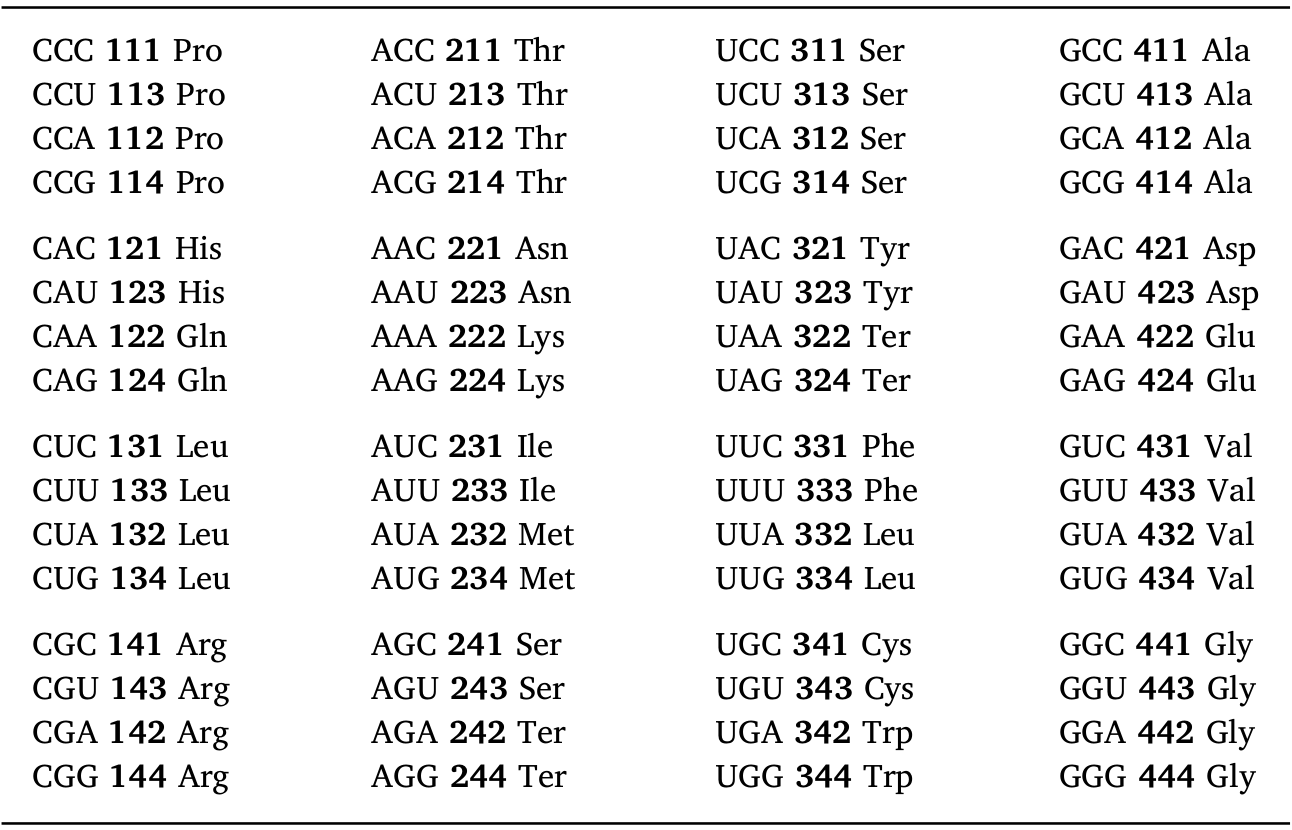
\includegraphics[width=1\textwidth]{slika8.jpeg}
  \caption{Dodela p-adičnih brojeva kodonima}
  \label{fig:my_label}
\end{figure}

\newpage
\begin{figure}[h!]
  \centering
  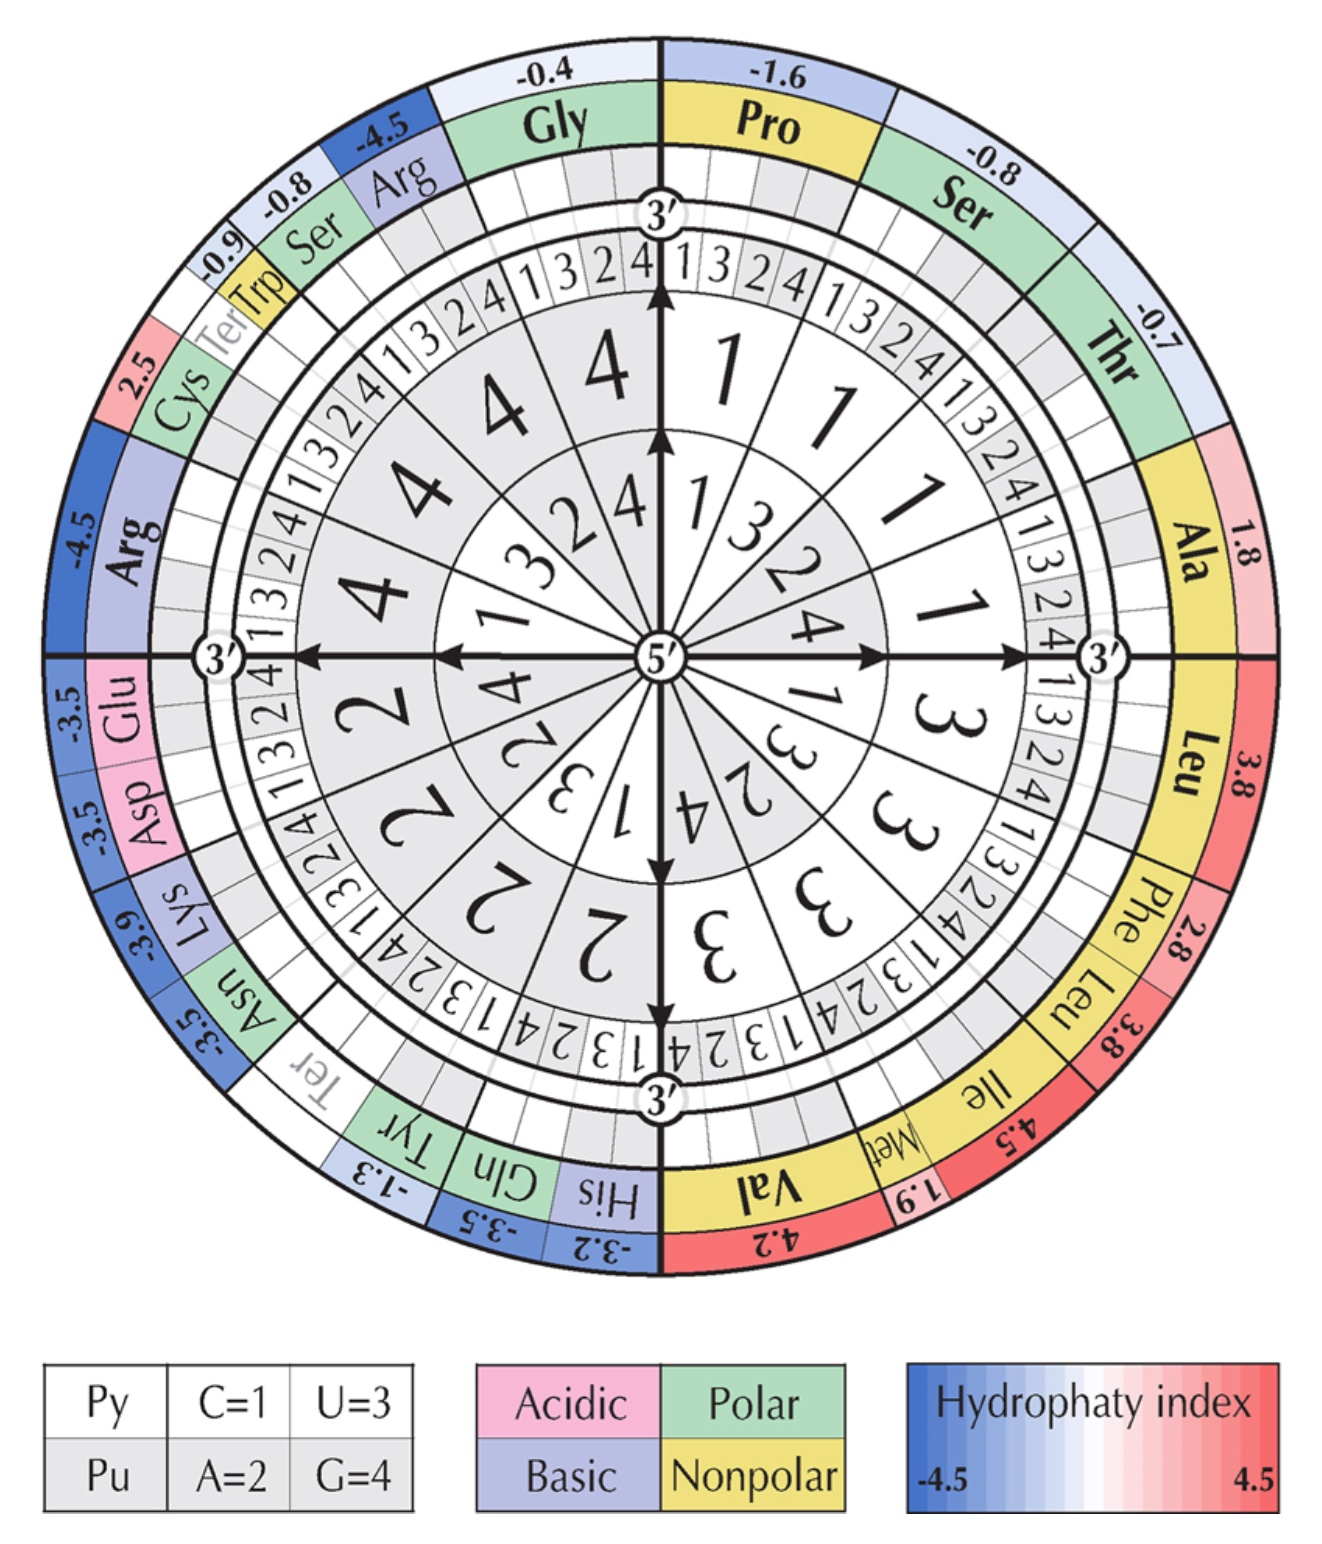
\includegraphics[width=0.46\textwidth]{slika9.jpeg}
  \caption{Standardni genetski kod preko p-adičnih brojeva}
  \label{fig:my_label}
  \vspace{0.5cm}
\end{figure}

Nakon što kodone prevedemo u p-adične brojeve, p-adično rastojanje možemo da izračunamo formulom:
\[
d_{5}(a, b) = \sum_{i=0}^{n} |a_{3i+1}a_{3i+2}a_{3i+3} - b_{3i+1}b_{3i+2}b_{3i+3}|_{5},
\]
gde su \(a\) i \(b\) dve RNK sekvence sa \(n+1\) kodona, \(n = 0, 1, 2, \ldots \)

\medskip
\begin{figure}[h!]
  \centering
  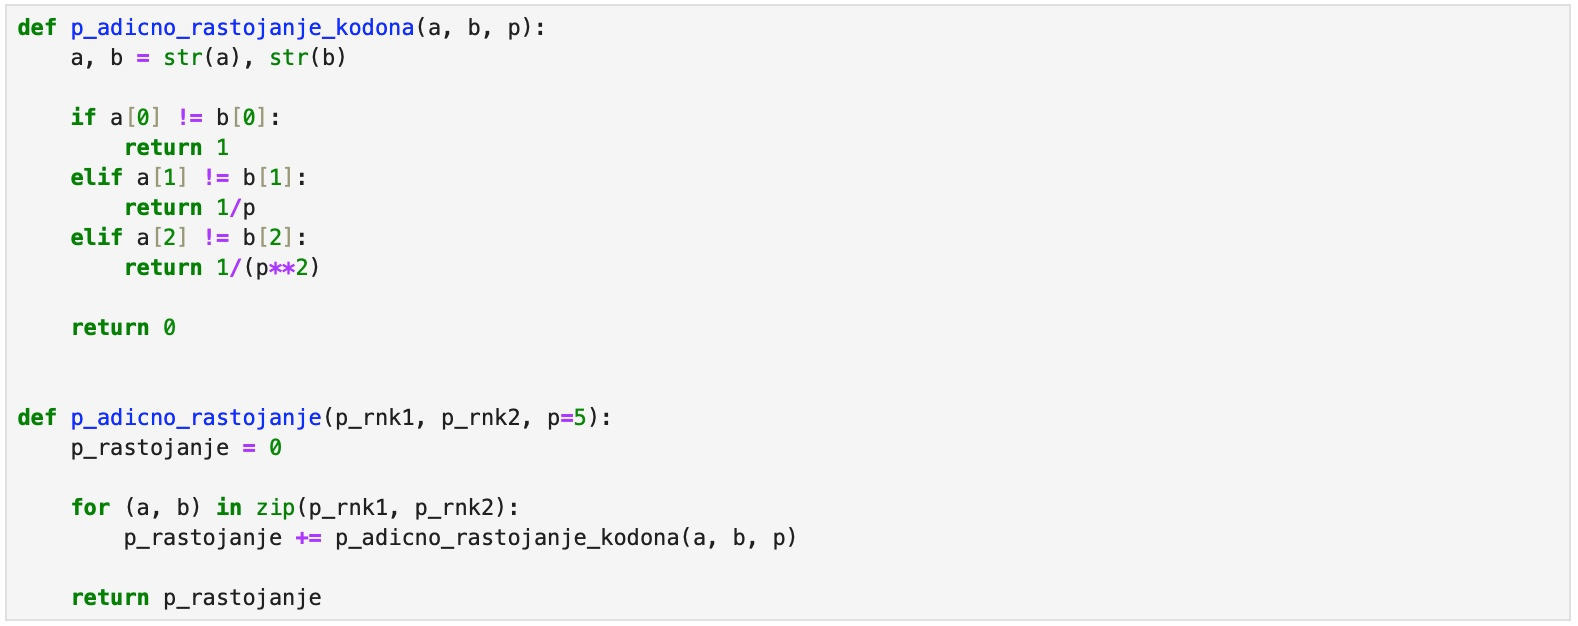
\includegraphics[width=1\textwidth]{slika10.jpeg}
  \caption{Funkcije za računanje p-adičnog rastojanja}
  \label{fig:my_label}
  \vspace{1cm}
\end{figure}

\newpage
\subsection{Hamingovo rastojanje}
Hamingovo rastojanje je metoda za merenje razlika između dve sekvence iste dužine. Ova metoda broji pozicije na kojima se odgovarajući simboli razlikuju. 

\medskip
U kontekstu genetskog koda, Hamingovo rastojanje se koristi za upoređivanje sekvenci DNK ili RNK. Postoje dva glavna pristupa primene Hamingovog rastojanja:
\begin{itemize}
    \item upoređivanje RNK sekvenci preko kodona: analizom se utvrđuje koliko se kodoni razlikuju na istim pozicijama u različitim RNK sekvencama. Ova metoda je korisna za identifikaciju mutacija ili varijacija u genetskim sekvencama koje mogu uticati na funkciju proteina.
    \item upoređivanje aminokiselina: fokus je na direktnom poređenju aminokiselina koje su kodirane kodonima. Promene u kodonima mogu dovesti do kodiranja istih aminokiselina, što može imati uticaj na strukturu, ali ne i na funkciju proteina. Upoređivanjem aminokiselina možemo bolje razumeti funkcionalne posledice genetiskih varijacija.
\end{itemize}

\begin{figure}[h!]
  \centering
  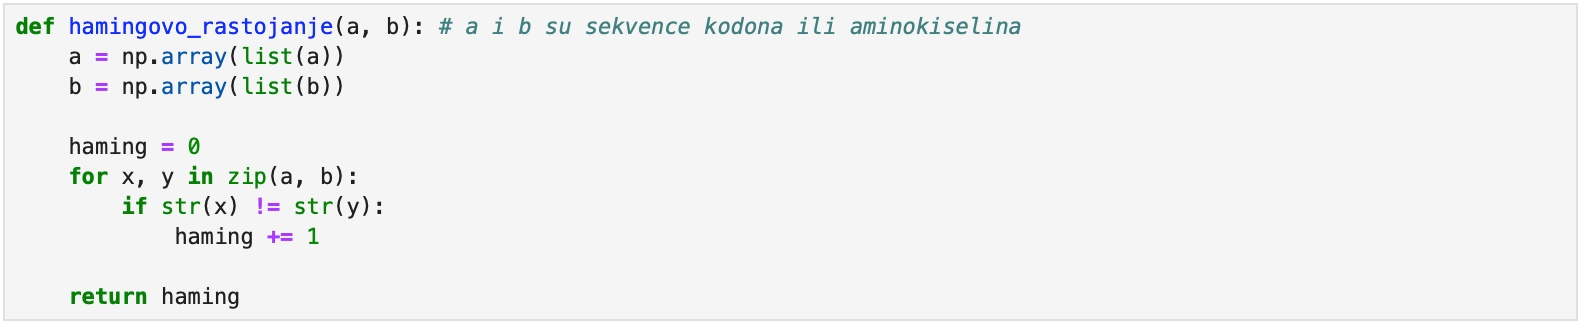
\includegraphics[width=1\textwidth]{slika11.jpeg}
  \caption{Funkcija za računanje Hamingovog rastojanja}
  \label{fig:my_label}
\end{figure}

\subsection{Analiza rezultata}
Kako bismo mogli da koristimo metode poput p-adičnog i Hamingovog rastojanja , sekvence koje se porede moraju da budu iste dužine. U ovom radu korišćena su dva načina dopunjavanja kraćih sekvenci:
\begin{enumerate}
    \item dopunjavanje najučestalijim kodonom: kraća sekvenca se dopunjava najučestalijim kodonom koji se pojavljuje u njoj do dužine duže sekvence.
    \item dopunjavanje najnajučestalijim nukleotidom: kraća sekvenca se dopunjava najučestalijim nukleotidom koji se pojavljuje u njoj do dužine duže sekvence.
\end{enumerate}
Dodatno, za računanje p-adičnog rastojanja koristili smo i treću metodu gde smo kraću sekvencu  nakon prevođenja u p-adične brojeve, dopunili “000".  Kako p-adična vrednost “000" ne postoji u standardnom genetskom kodu, to predstavlja dobar indikator da su na tim pozicijama sekvence različite.

\bigskip
\noindent
\textbf{Dobijeni rezultati računanjem p-adičnog rastojanja:}
\bigskip

\begin{figure}[h!]
  \centering
  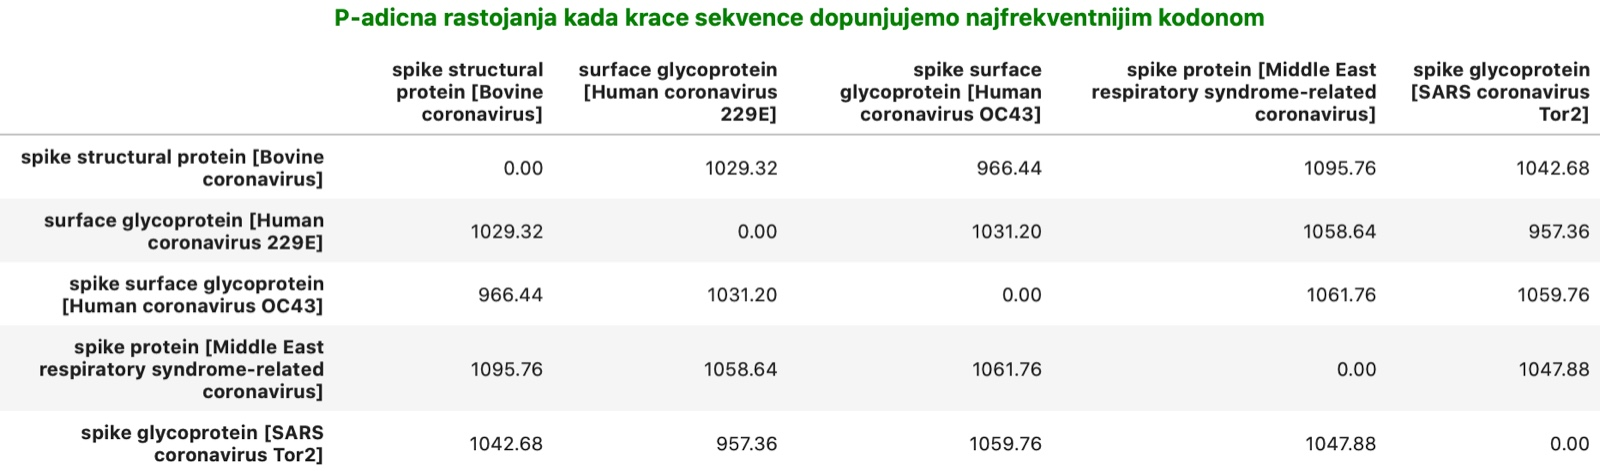
\includegraphics[width=1.0\textwidth]{slika12.jpeg}
  \caption{P-adična rastojanja nakon dopune najučestalijim kodonom}
  \label{fig:my_label}
\end{figure}

\begin{figure}[h!]
  \centering
  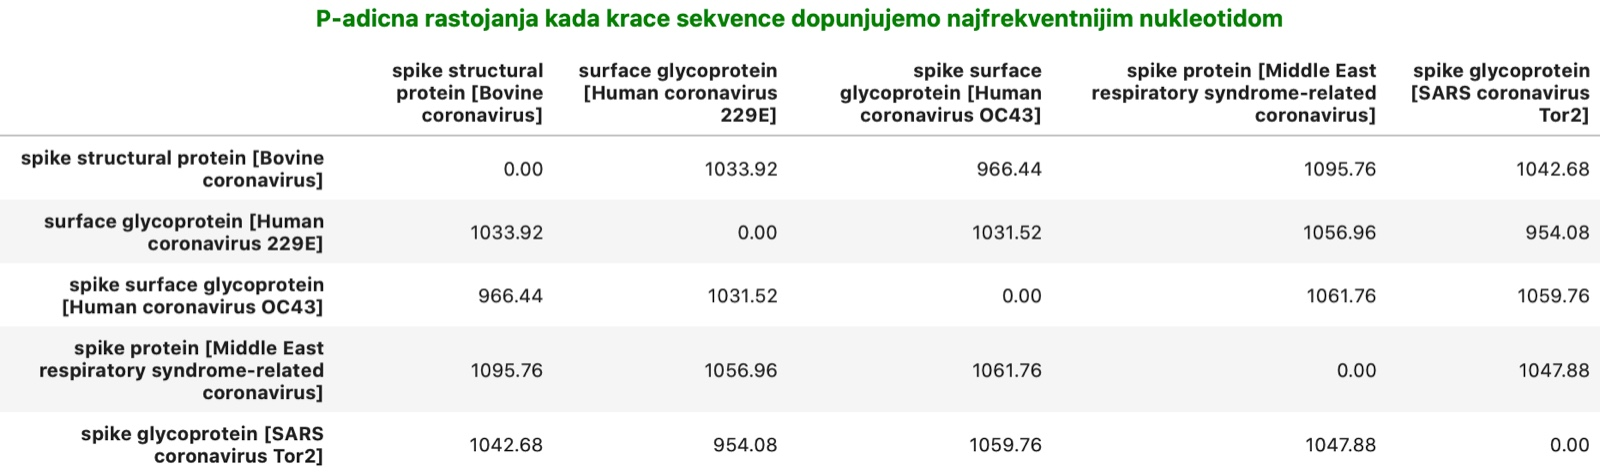
\includegraphics[width=1.0\textwidth]{slika13.jpeg}
  \caption{P-adična rastojanja nakon dopune najučestalijim nukleotidom}
  \label{fig:my_label}
\end{figure}

\begin{figure}[h!]
  \centering
  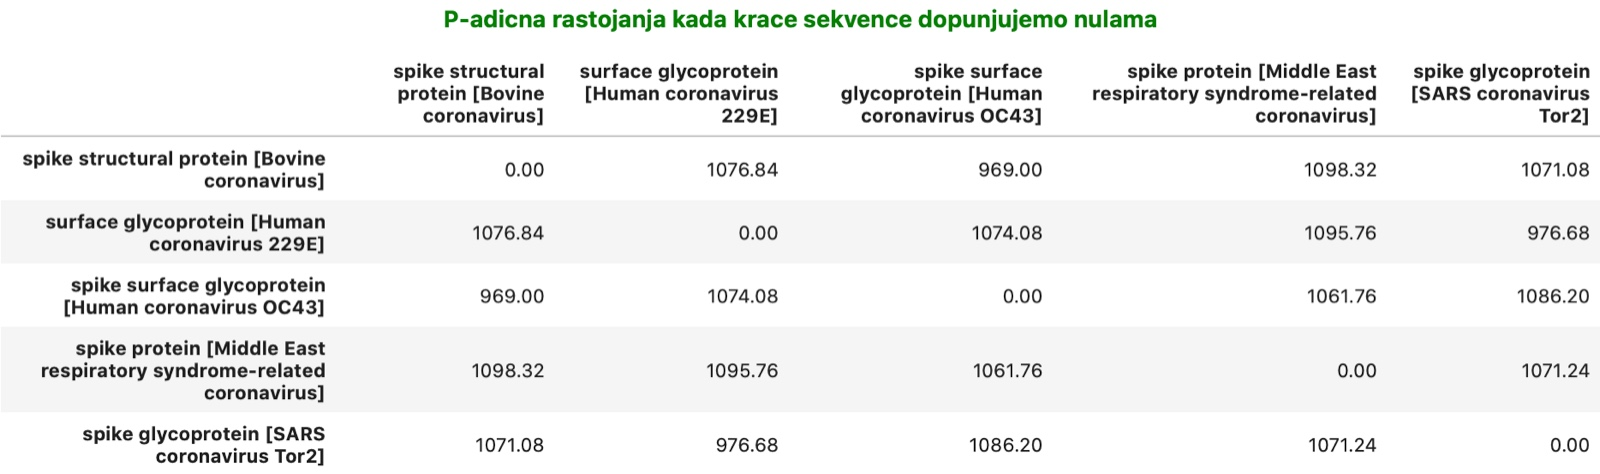
\includegraphics[width=1.0\textwidth]{slika14.jpeg}
  \caption{P-adična rastojanja nakon dopune nulama}
  \label{fig:my_label}
\end{figure}

\bigskip
\noindent
\textbf{Dobijeni rezultati računanjem Hamingovog rastojanja poredivši kodone:}
\bigskip

\begin{figure}[h!]
  \centering
  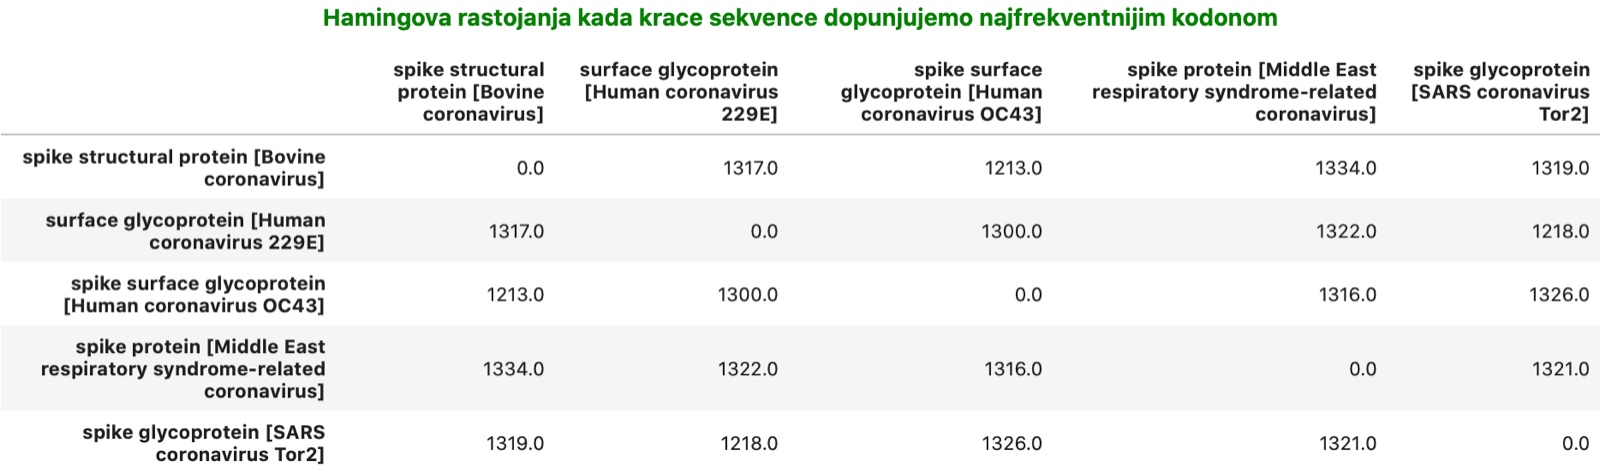
\includegraphics[width=1.0\textwidth]{slika15.jpeg}
  \caption{Hamingova rastojanja nakon dopune najučestalijim kodonom}
  \label{fig:my_label}
\end{figure}

\begin{figure}[h!]
  \centering
  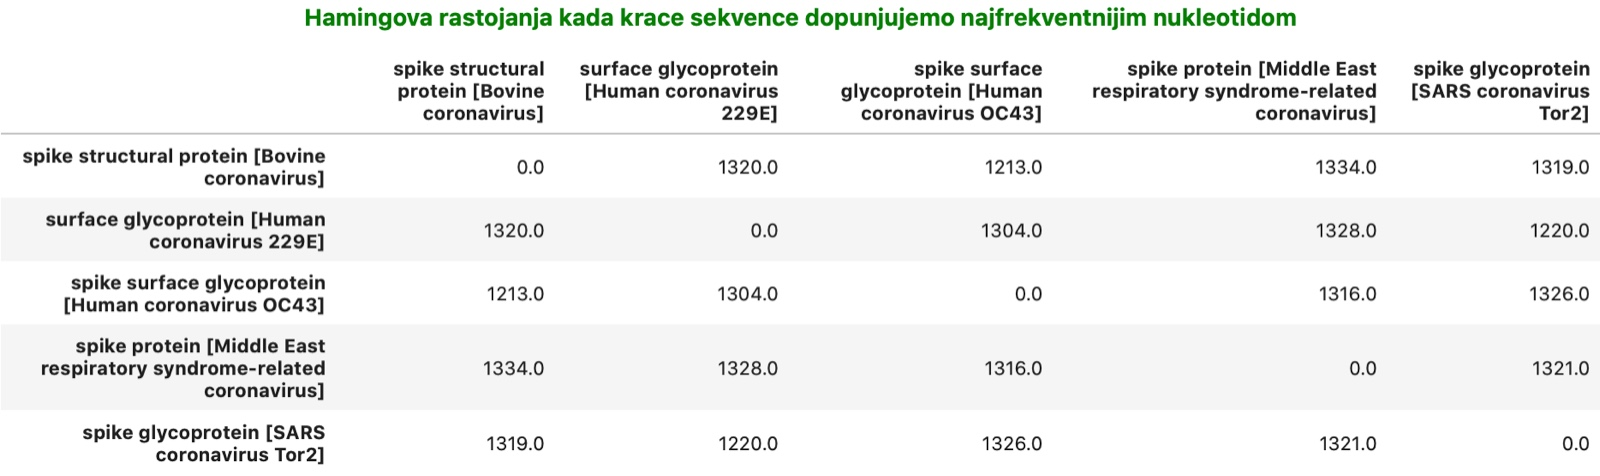
\includegraphics[width=1.0\textwidth]{slika16.jpeg}
  \caption{Hamingova rastojanja nakon dopune najučestalijim nukleotidom}
  \label{fig:my_label}
\end{figure}

\bigskip
\noindent
\textbf{Dobijeni rezultati računanjem Hamingovog rastojanja poredivši aminokiseline:}
\bigskip

\begin{figure}[h!]
  \centering
  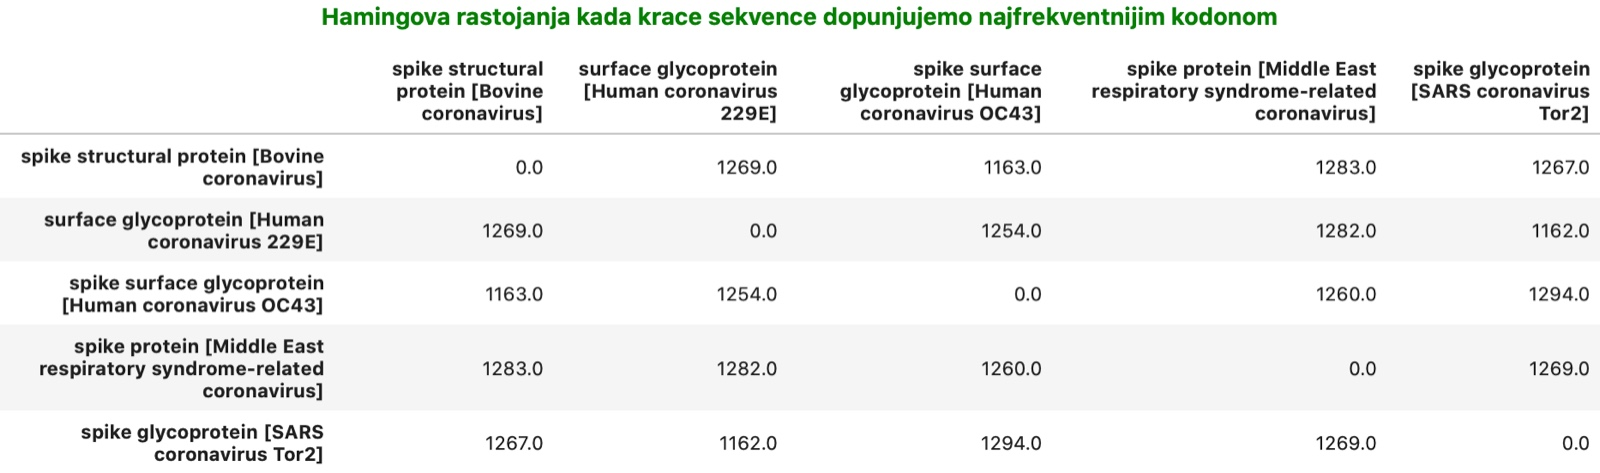
\includegraphics[width=1.0\textwidth]{slika17.jpeg}
  \caption{Hamingova rastojanja nakon dopune najučestalijim kodonom}
  \label{fig:my_label}
\end{figure}

\begin{figure}[h!]
  \centering
  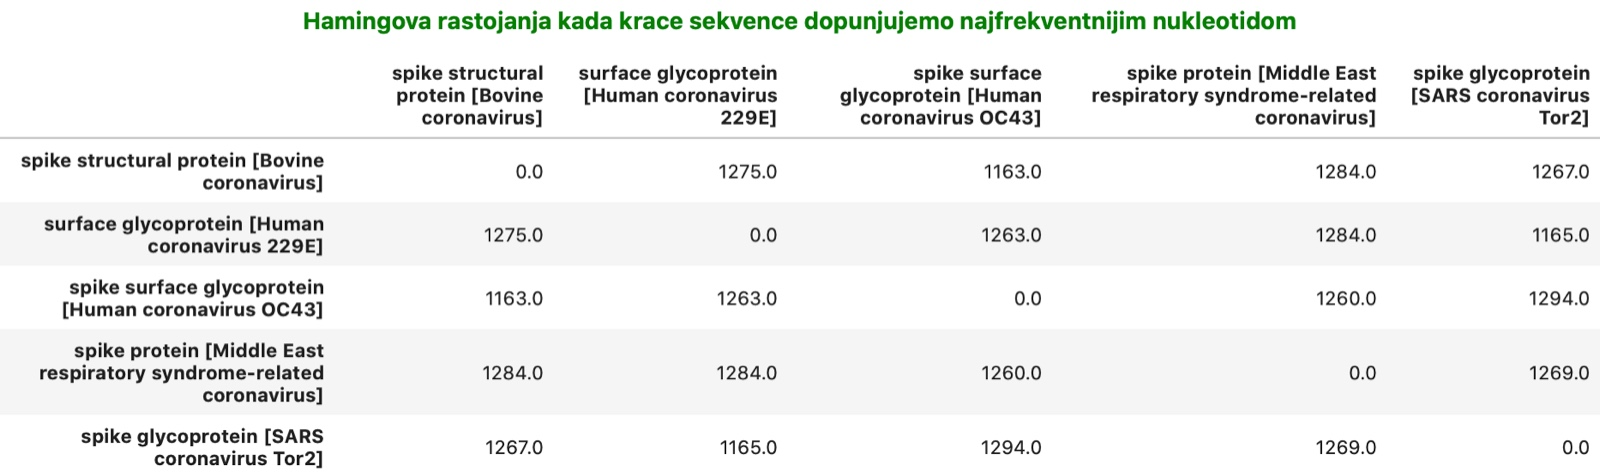
\includegraphics[width=1.0\textwidth]{slika18.jpeg}
  \caption{Hamingova rastojanja nakon dopune najučestalijim nukleotidom}
  \label{fig:my_label}
\end{figure}

\bigskip
Ono što prvo možemo primetiti jesu slični obrasci u rastojanjima između površinskih proteina koronavirusa, što ukazuje na pouzdanost naše analize, nezavisno od specifične metode dopunjavanja kraćih sekvenci. Ovo je važno jer pokazuje da rezultati analize ostaju konzistentni i relevantni bez obzira na sitnije razlike u metodama obrade podataka.

\medskip
Takođe, primećujemo da su rastojanja dobijena Hamingovim rastojanjem nešto veća u odnosu na rastojanja dobijena p-adičnim rastojanjem, što se može objasniti razlikama u načinu funkcionisanja ovih metrika. P-adična rastojanja uzimaju u obzir poziciju prve razlike u nukleotidima unutar kodona, dok Hamingova rastojanja jednostavno broje pozicije na kojima su kodoni različiti, bez obzira na važnost tih razlika. 

Ove razlike ukazuju na to da Hamingova rastojanja pružaju grublju sliku sličnosti, dok p-adična rastojanja daju detaljniji uvid u specifične evolucione promene.

\medskip
Kada poredimo aminokiseline umesto kodona, dobijamo manja rastojanja. Ovo je očekivano jer različiti kodoni mogu kodirati istu aminokiselinu (degeneracija genetskog koda), smanjujući broj pozicija na kojima su sekvence različite. 

\bigskip
Analizom rezultata, vidimo da postoje nekoliko parova proteina koji pokazuju veću sličnost:
\begin{itemize}
    \item Spike structural protein [Bovine coronavirus] i Spike surface glycoprotein [Human coronavirus OC43].
    \item Spike glycoprotein [SARS coronavirus Tor2] i Surface glycoprotein [Human coronavirus 229E].
\end{itemize}
Bliskost između površinskih proteina Bovine coronavirusa i Human coronavirusa OC43 je razumljiva jer oba virusa pripadaju istoj virusnoj grupi beta-koronavirusa i za ulazak u ćeliju domaćina koriste dodatno HE protein. Slično, bliskost između SARS-CoV-1 i Human coronavirusa 229E može biti povezana sa sličnim mehanizmima interakcije sa receptorima domaćina.

\medskip
Međutim, veću razliku u rastojanjima ima protein:
\begin{itemize}
    \item Spike protein [Middle East respiratory syndrome-related coronavirus] sa spike proteinima ostalih koronavirusa.
\end{itemize}
Ove udaljenosti se mogu objasniti različitim evolutivnim stazama i funkcionalnim adaptacijama koje su ovi virusi prošli. MERS-CoV je poznat po svojoj specifičnosti prema DPP4 receptoru, dok većina ostalih beta-koronavirusi koriste ACE2 ili slične receptore, što ukazuje na značajne razlike u strukturi i funkciji njihovih spike proteina.

\newpage
\section{Klasterovanje}
Nakon analize sličnosti među površinskim proteinima koronavirusa korišćenjem p-adičnog i Hamingovog rastojanja, sada prelazimo na analizu kroz primenu edit rastojanja i klasterovanja. Kroz ovaj proces, cilj nam je da identifikujemo zajedničke karakteristike i evolutivne veze među proteinima.

\subsection{Edit rastojanje}
Edit rastojanje meri razliku između dva niza karaktera određujući minimalan broj operacija (umetanja, brisanja, zamene) potrebnih za pretvaranje jednog niza u drugi. Dinamičko programiranje omogućava efikasno pronalaženje najkraćeg niza operacija, precizno mereći razlike čak i između sekvenci različitih dužina. 

\medskip
U bioinformatičkim istraživanjima, edit rastojanje je ključan alat za razumevanje genetskih promena, evolutivnih odnosa i funkcionalnih sličnosti među različitim organizmima ili sekvencama.


\bigskip
\begin{figure}[h!]
  \centering
  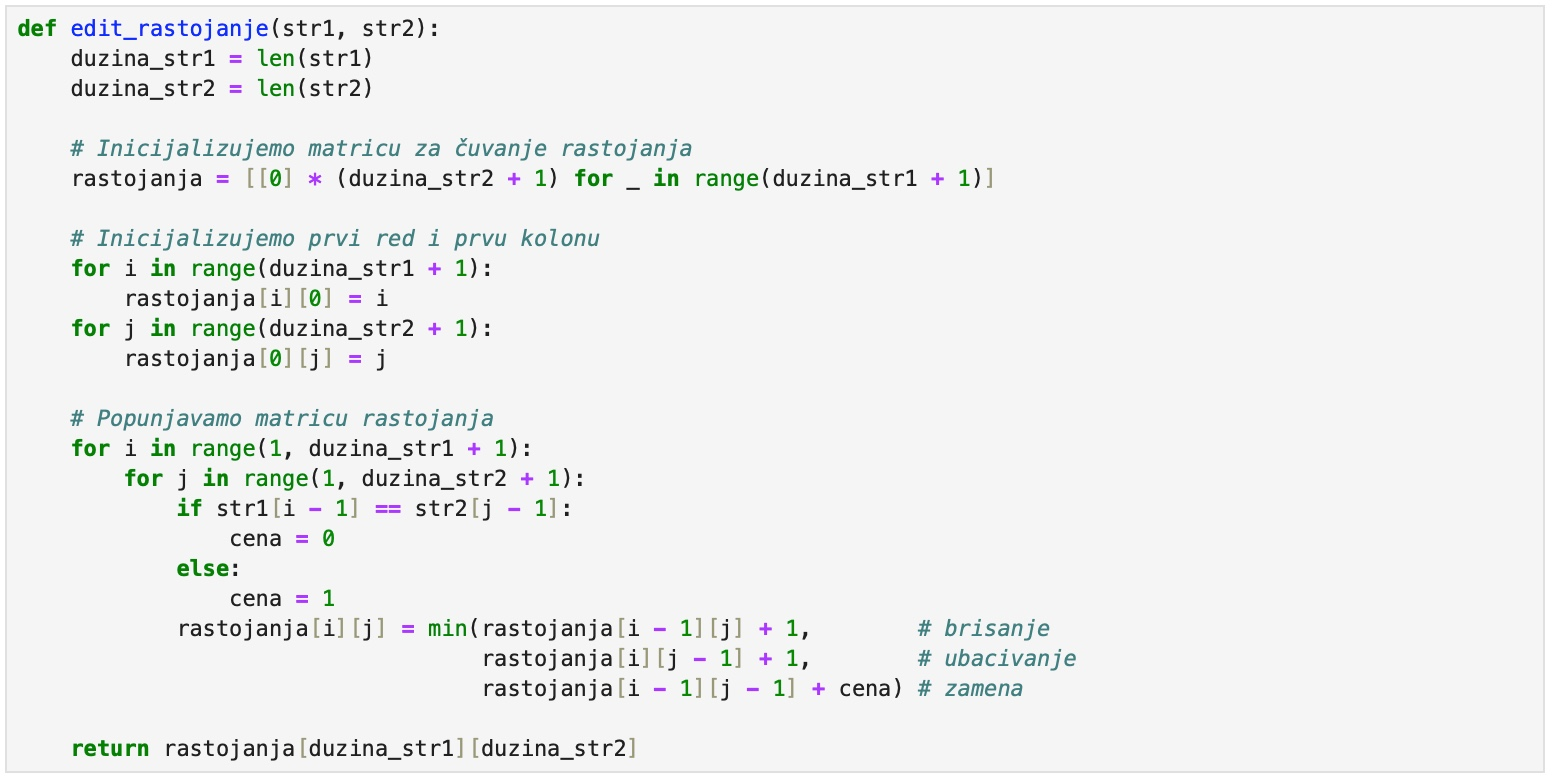
\includegraphics[width=1\textwidth]{slika19.jpeg}
  \caption{Funkcija za računanje edit rastojanja}
  \label{fig:my_label}
\end{figure}

\bigskip
Kod za računanje edit rastojanja se nalazi u \texttt{edit\_rastojanje.ipynb} datoteci, a dobijeni rezultati zabeleženi su u \texttt{edit\_rastojanja.txt} datoteci.

\medskip
Ukupan broj referentnih proteina za naših pet koronavirusa iznosi 56. Za svaku RNK sekvencu koja kodira protein, vršimo poređenje sa svakom drugom, što dovodi do ukupno 1540 kombinacija za računanje edit rastojanja. S obzirom na to da nekoliko sekvenci ima dužinu veću od 20000 nukleotida, proces računanja edit rastojanja bio je dugotrajan i zahtevan i završen je nakon 14 sati. Zbog ove složenosti, ne preporučujemo da pokrećete ovaj kod.


\subsection{Hijerarhijsko sakupljajuće klasterovanje}
Hijerarhijsko sakupljajuće klasterovanje (engl. Hierarchical Agglomerative Clustering) je tehnika koja grupiše podatke u hijerarhijsku strukturu. Ova tehnika počinje sa svakim podatkom kao odvojenim klasterom i zatim iterativno spaja najbliže klastere dok ne ostane samo jedan klaster koji sadrži sve podatke.

\medskip
Ključni korak u analizi hijerarhijskog sakupljajućeg klasterovanja je interpretacija dendrograma, grafičke reprezentacije hijerarhijske strukture klastera. Dendrogram prikazuje način na koji su podaci grupisani u klastere i omogućava vizuelnu analizu sličnosti među grupama.

\bigskip
Nakon što smo dobili matricu rastojanja koristeći edit rastojanje kao meru sličnosti između svakog para proteina, primenili smo algoritam hijerarhijskog sakupljajućeg klasterovanja na osnovu ove matrice kako bismo grupisali proteine u klastere. 

\bigskip
\begin{figure}[h!]
  \centering
  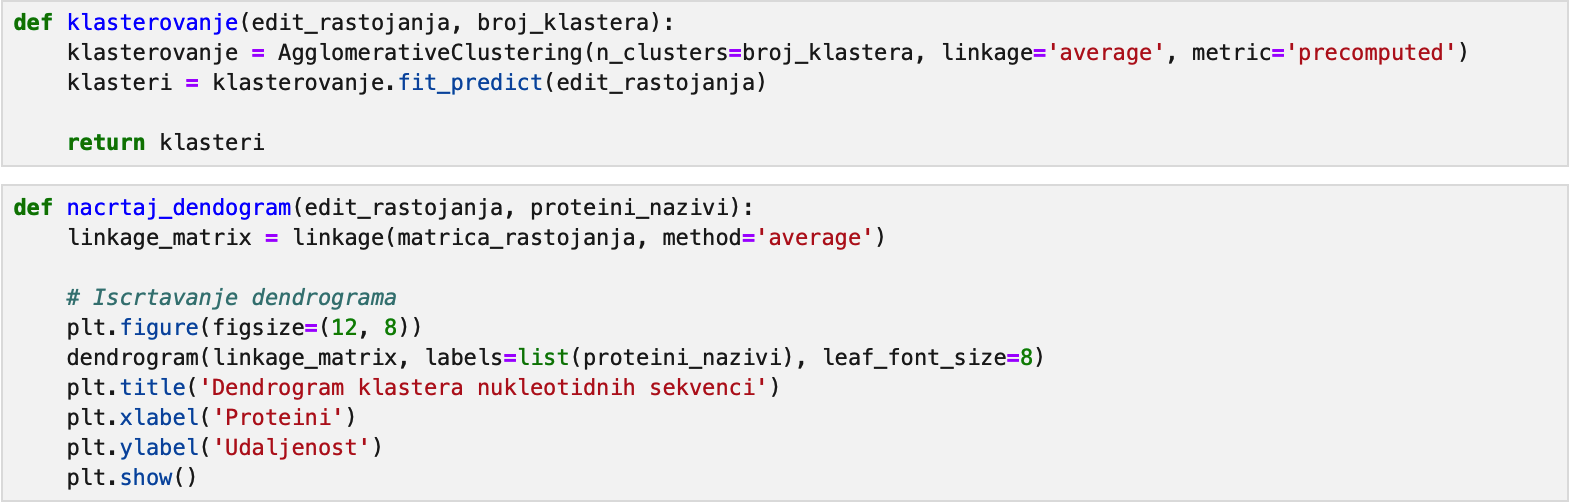
\includegraphics[width=1.0\textwidth]{slika20.jpeg}
  \caption{Funkcije za klasterovanje podataka i crtanje dendograma}
  \label{fig:my_label}
\end{figure}

\bigskip
Ceo kod se nalazi u datoteci \texttt{hijerarhijsko\_klasterovanje.ipynb}.

\newpage
\begin{figure}[h!]
  \hspace*{-1.3cm}
  \centering
  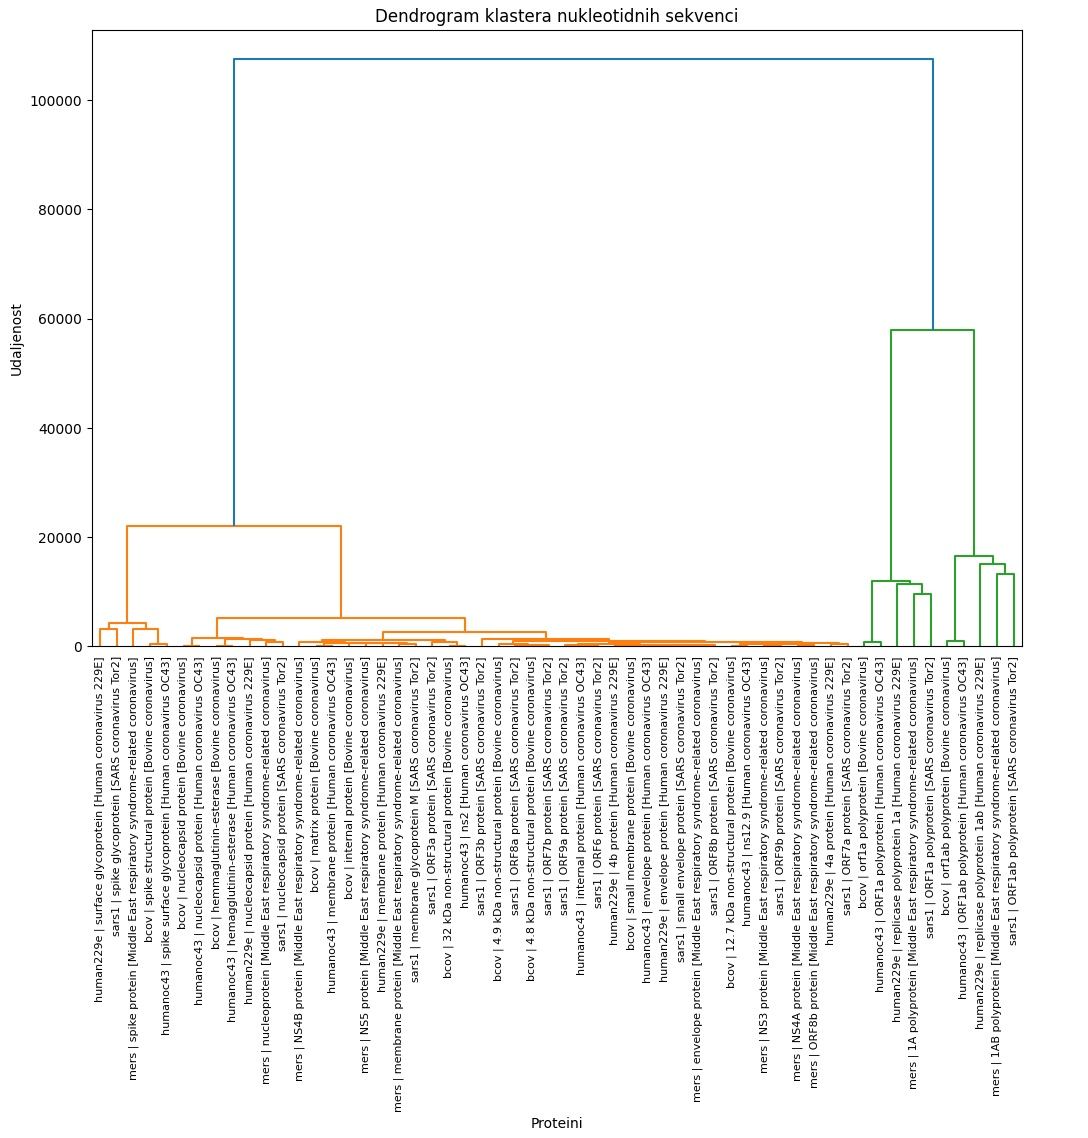
\includegraphics[width=1.2\textwidth]{slika21.jpeg}
  \caption{Dendrogram klastera}
  \label{fig:my_label}
\end{figure}

\bigskip
Nakon detaljne analize dendrograma, zaključili smo da postoji podela na tri glavne grupe, što je rezultiralo odlukom da koristimo tri klastera kao optimalan broj.


\subsection{Vizuelizacija klastera}
Kako bismo dobijene klasterovane podatke vizuelizovali i bolje ih razumeli, primenili smo analizu glavnih komponenti (engl. Principal Component Analysis - PCA) na matricu edit rastojanja. 

\medskip
PCA je tehnika smanjivanja dimenzionalnosti koja transformiše originalne podatke u novi skup linearno nezavisnih promenljivih, poznatih kao glavne komponente, koje zadržavaju maksimalnu varijansu podataka.

\bigskip
\begin{figure}[h!]
  \centering
  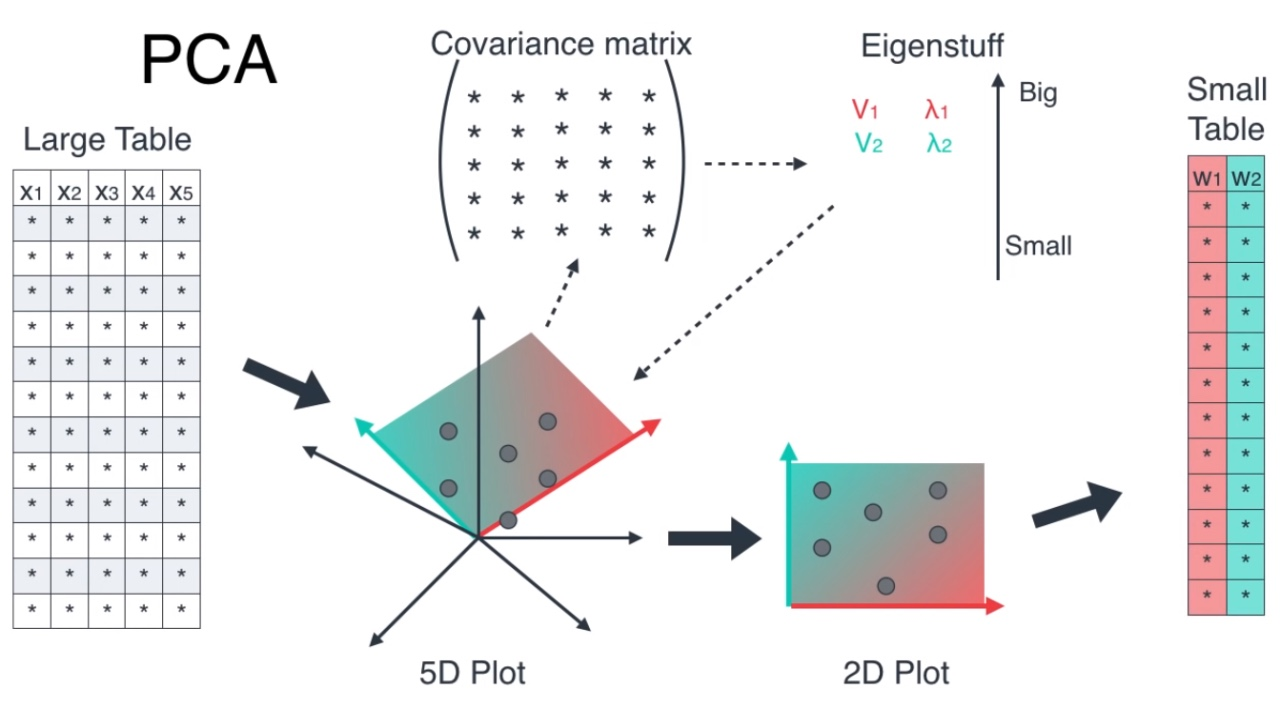
\includegraphics[width=0.7\textwidth]{slika22.jpeg}
  \caption{Princip smanjenja dimezionalnosti podataka}
  \label{fig:my_label}
\end{figure}

\bigskip
Primena PCA na matricu edit rastojanja omogućila je smanjenje dimenzionalnosti na dve glavne komponente, čime smo postigli dvodimenzionalnu reprezentaciju podataka. Ova dvodimenzionalna matrica omogućava nam vizualizaciju klastera u dvodimenzionalnom prostoru i lakšu identifikaciju obrasca i grupisanja među proteinima.

\bigskip
Interaktivnu vizuelizaciju klastera možete pogledati u datoteci \texttt{klasteri.html}, a sliku istog u nastavku.

\newpage
\begin{figure}[h!]
  \centering
  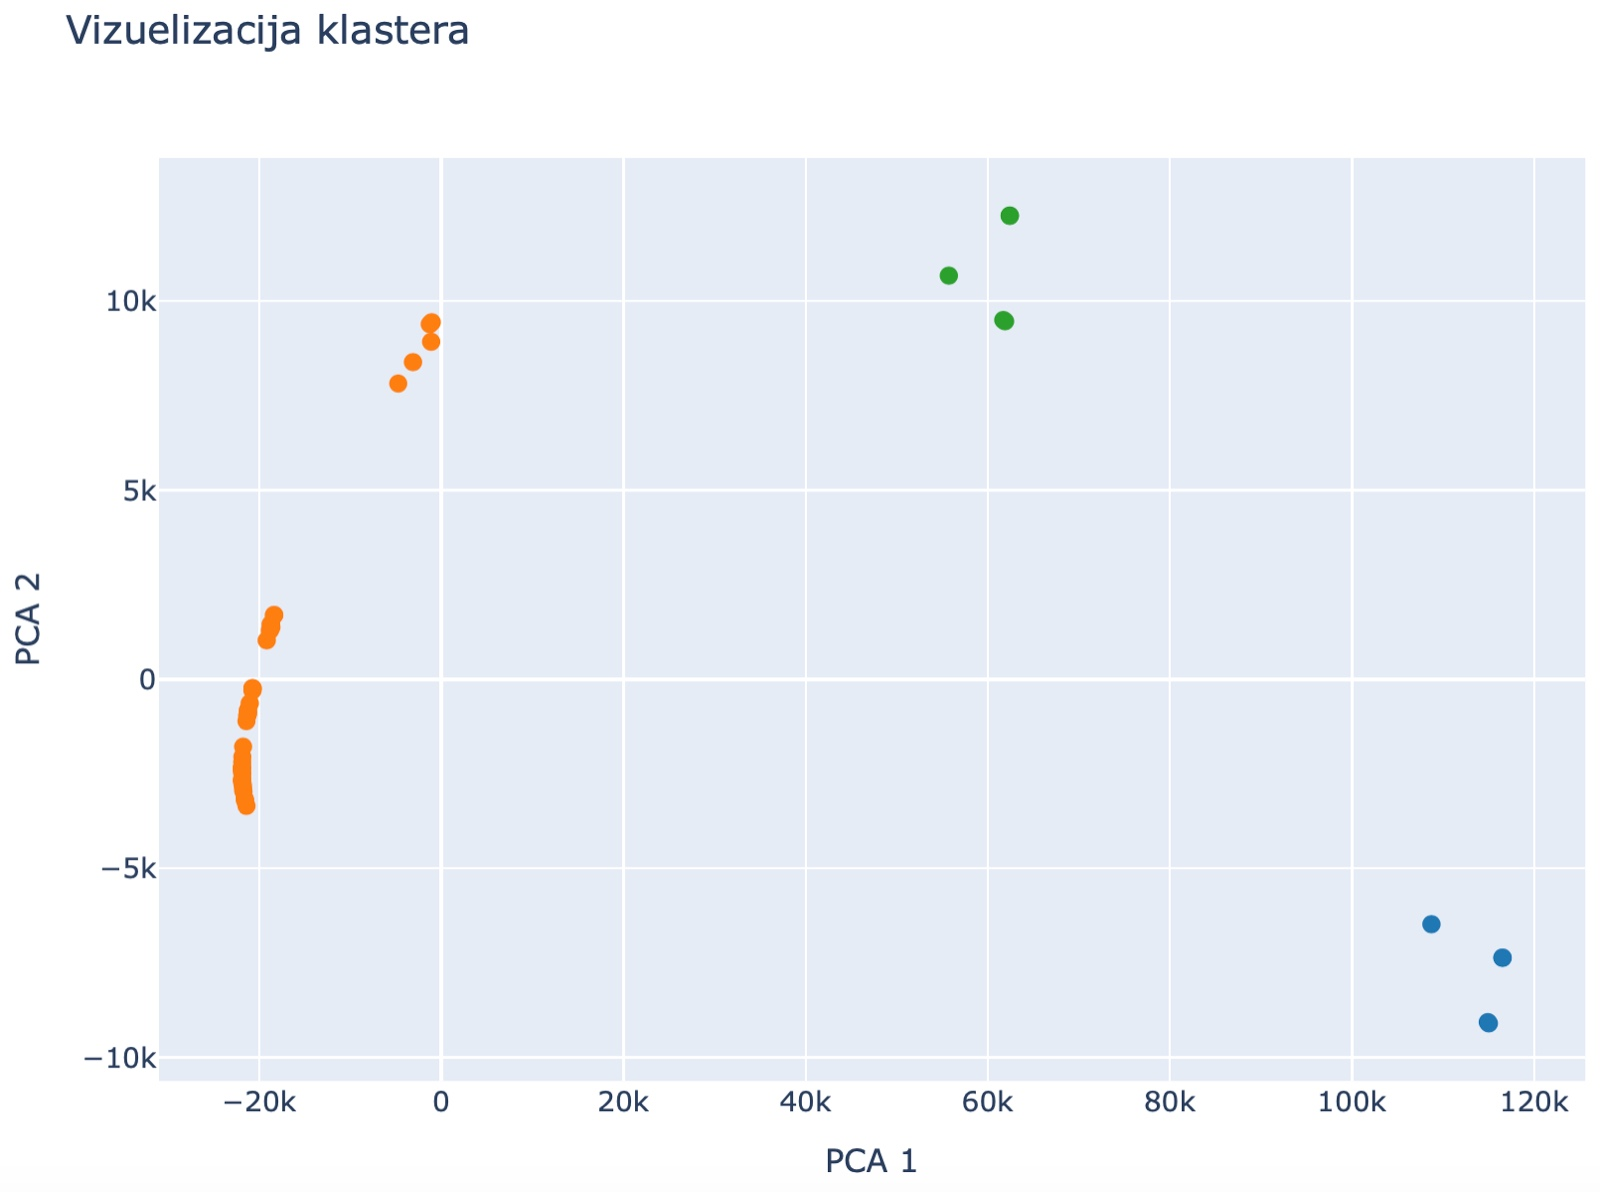
\includegraphics[width=1\textwidth]{slika23.jpeg}
  \caption{Vizuelizacija klastera}
  \label{fig:my_label}
\end{figure}

\bigskip
Na osnovu vizuelizacije klastera, možemo zaključiti sledeće:
\begin{itemize}
    \item U zelenom klasteru nalaze se ORF1a polyprotein koronavirusa SARS-CoV-1, BCoV i HCoV-OC43, 1A polyprotein MERS-CoV-a i replicase polyprotein 1a virusa HCoV-229E. Ovi proteini su deo ne-strukturnih proteina koji su ključni za replikaciju i sintezu virusnog RNK genoma i proteina.
    \item Plavi klaster obuhvata proteine: ORF1ab i 1AB polyproteine i replicase polyprotein 1ab. Kao i proteini u zelenom klasteru, ovi proteini su ne-strukturni i osnovni za procese transkripcije i replikacije virusne RNK.
    \item Narandžasti klaster obuhvata raznovrsne proteine koji su ključni za različite aspekte životnog ciklusa koronavirusa. On sadrži proteine različitih funkcija i struktura, ali njihovo grupisanje zajedno ukazuje na određene zajedničke karakteristike. 
    \newpage
    Ovaj klaster uključuje: 
    \begin{itemize}
        \item Ne-strukturne proteine (NS3 protein, NS4A protein, NS4B protein, NS5 protein) koji su ključni za replikaciju virusa i modulaciju imunskog odgovora domaćina. 
        \item Strukturne proteine poput envelope proteina, membrane proteina i nucleocapsid proteina, koji su važni za formiranje strukture virusnih čestica i održavanje njihovog integriteta.
        \item Površinske proteine, koji se grupišu u jednom podklasteru.
    \end{itemize}

    Pored ovih, narandžasti klaster uključuje i ostale proteine koji mogu imati različite uloge u infekciji, replikaciji i patogenezi virusa. Njihovo zajedničko grupisanje sugeriše da, uprkos funkcionalnoj raznolikosti, dele određene evolutivne ili strukturne karakteristike koje ih čine sličnijima jedne drugima u poređenju sa proteinima iz drugih klastera.
\end{itemize}

\bigskip
Posebno je važno napomenuti da su proteini koji imaju slične funkcije, iako potiču od različitih koronavirusa, međusobno bliži nego proteini sa različitim funkcijama.

\bigskip
Da li zaista postoji podklaster ili se pojavljuje samo vizuelno zbog PCA?

\smallskip
Smanjenje dimenzionalnosti može dovesti do pojave da su neki podaci grupisani ili razdvojeni na način koji nije u potpunosti u skladu sa biologijom. 
U kontekstu analize površinskih proteina koronavirusa, iako možemo primetiti određene obrasce grupisanja koristeći PCA, važno je imati na umu da slika koju dobijamo malo iskrivljena. Ipak, smanjenjem dimenzionalnosti se jasno izdvajio podklaster površinskih proteina, što ukazuje na to da zaista postoji stvarna biološka osnova za tu grupaciju.

\smallskip
Osim toga, dendrogram potvrđuje grupisanje površinskih proteina u određen podklaster (videdti sliku 21), što je dodatna podrška postojanju takve grupacije. 


\bigskip
Kada bismo “uveličali" podklaster u kome se nalaze površinski proteini, mogli bismo detaljnije videti njihovu raspodelu. Međutim, ovo je raspored prikazan na matrici na koju je primenjena PCA, čime je smanjena njena dimenzija sa 56x56 na 56x2.

\newpage
\begin{figure}[h!]
  \centering
  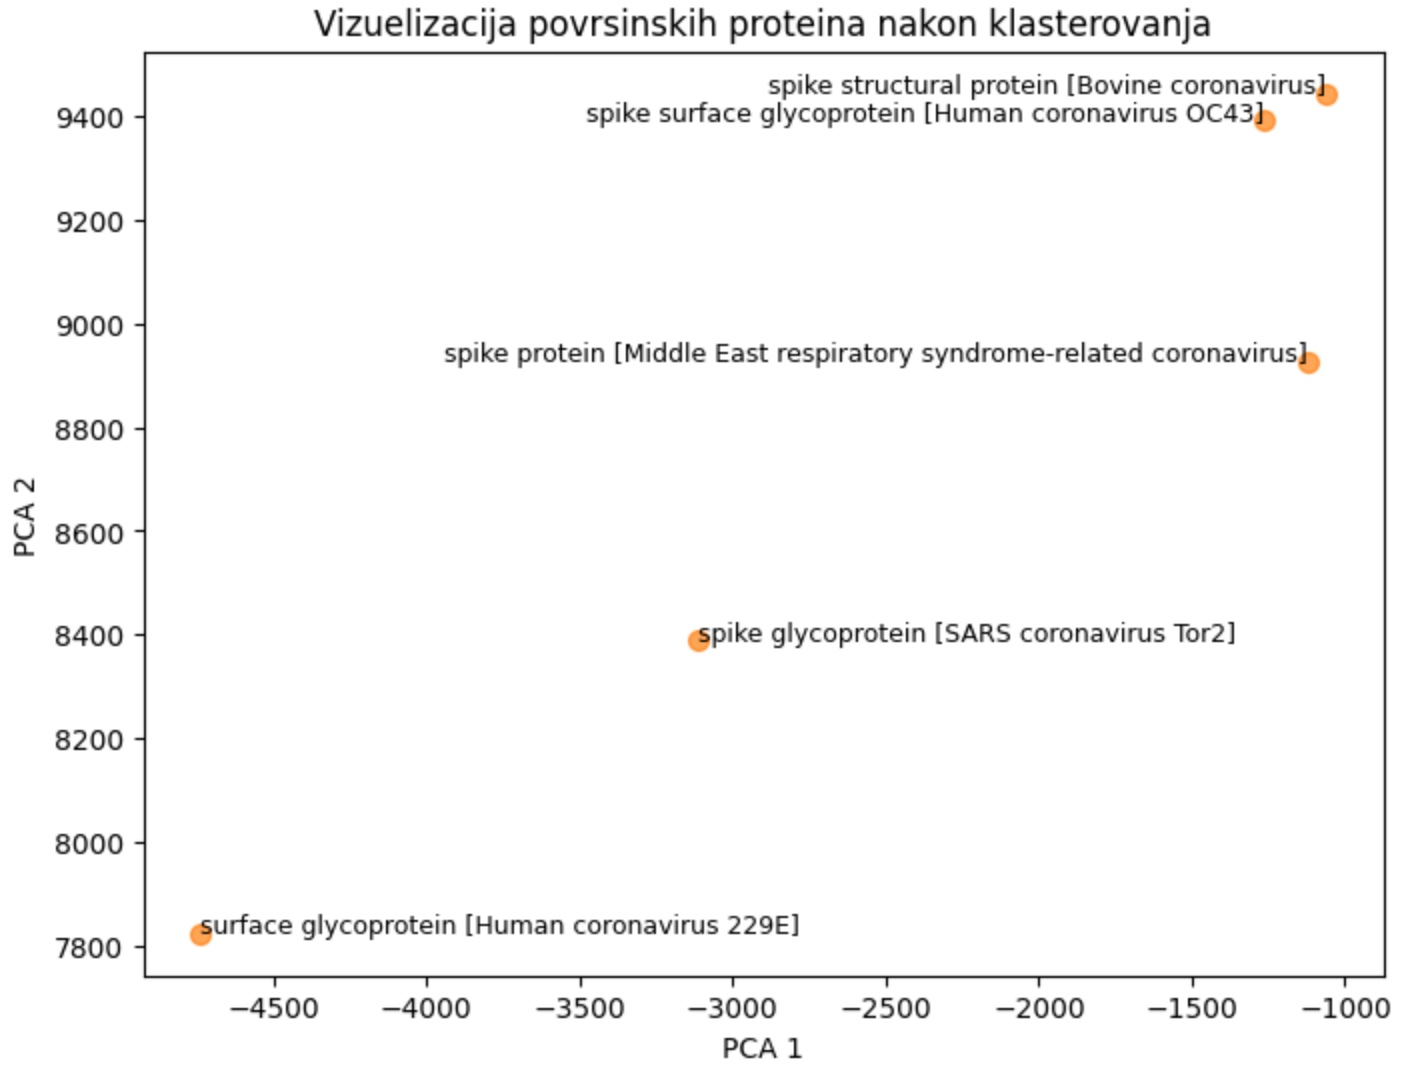
\includegraphics[width=1\textwidth]{slika24.jpeg}
  \caption{Vizuelizacija podklastera}
  \label{fig:my_label}
\end{figure}

\bigskip
\noindent
\textbf{Dobijeni rezultati računanjem edit rastojanja (prikaz samo za površinske proteine):}

\bigskip
\begin{figure}[h!]
  \centering
  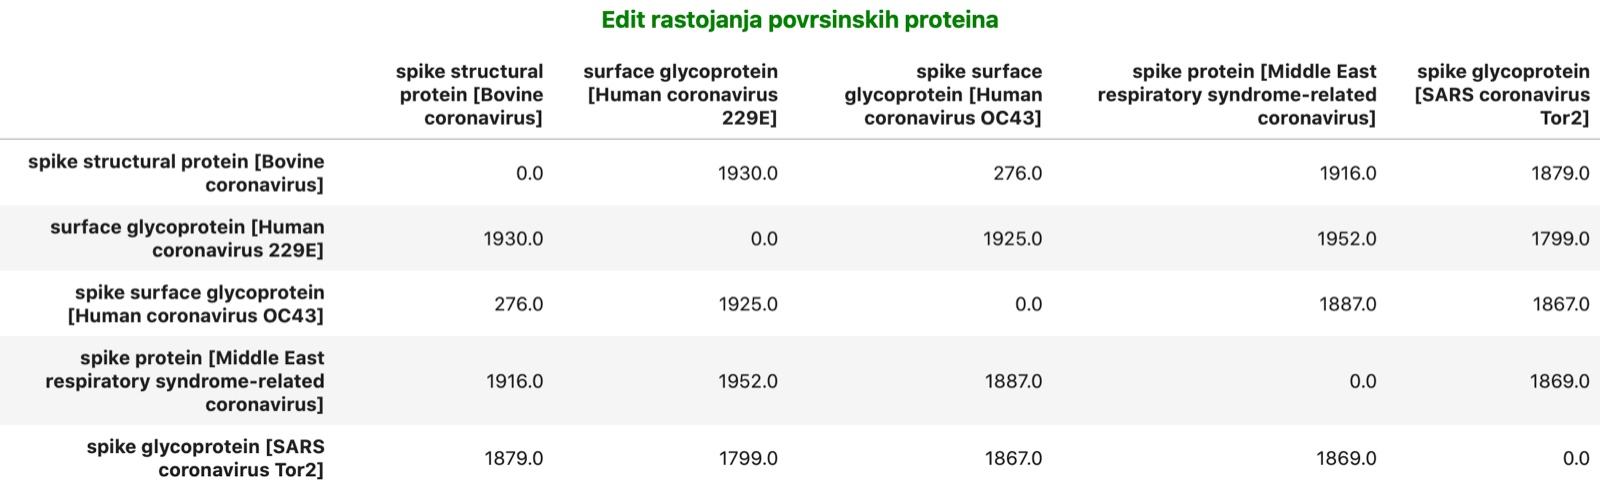
\includegraphics[width=1\textwidth]{slika25.jpeg}
  \caption{Edit rastojanja}
  \label{fig:my_label}
\end{figure}

\newpage
\subsection{Poređenje rezultata površinskih proteina sa p-adičnim rastojanjem}
Kako bismo bolje i preciznije mogli vizuelno da uporedimo rezultate klasterovanja i računanja edit rastojanja sa p-adičnim rastojanjem, napravili smo novu matricu koja sadrži samo edit rastojanja između površinskih proteina. Na tako dobijenu matricu smo primenili PCA radi vizuelizacije. Takođe, PCA smo primenili i na jednu od matrica p-adičnih rastojanja (u datoteci \texttt{povrsinski\_proteini\_rastojanja.ipynb}). Ovim smo obezbedili smanjenje dimenzionalnosti oba skupa podataka sa 5x5 na 5x2 i dobili sličnije iskrivljenje slika zbog PCA.

\bigskip
\begin{figure}[h!]
  \centering
  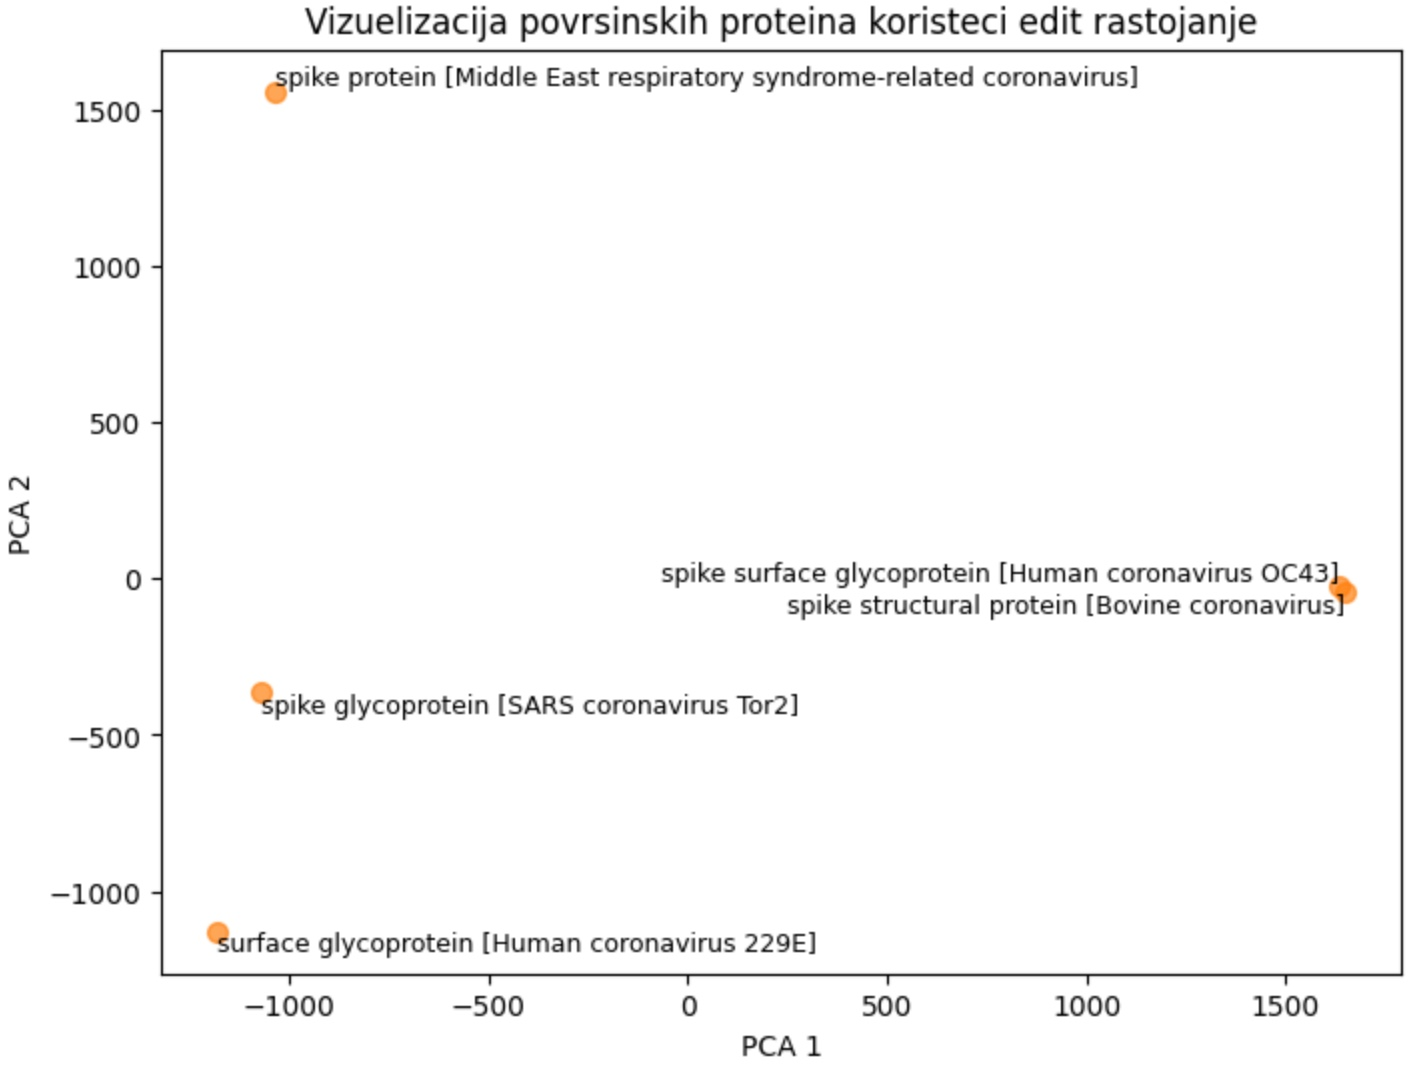
\includegraphics[width=1\textwidth]{slika26.jpeg}
  \caption{Vizuelizacija površinskih proteina koristeći edit rastojanje}
  \label{fig:my_label}
\end{figure}

\begin{figure}[h!]
  \centering
  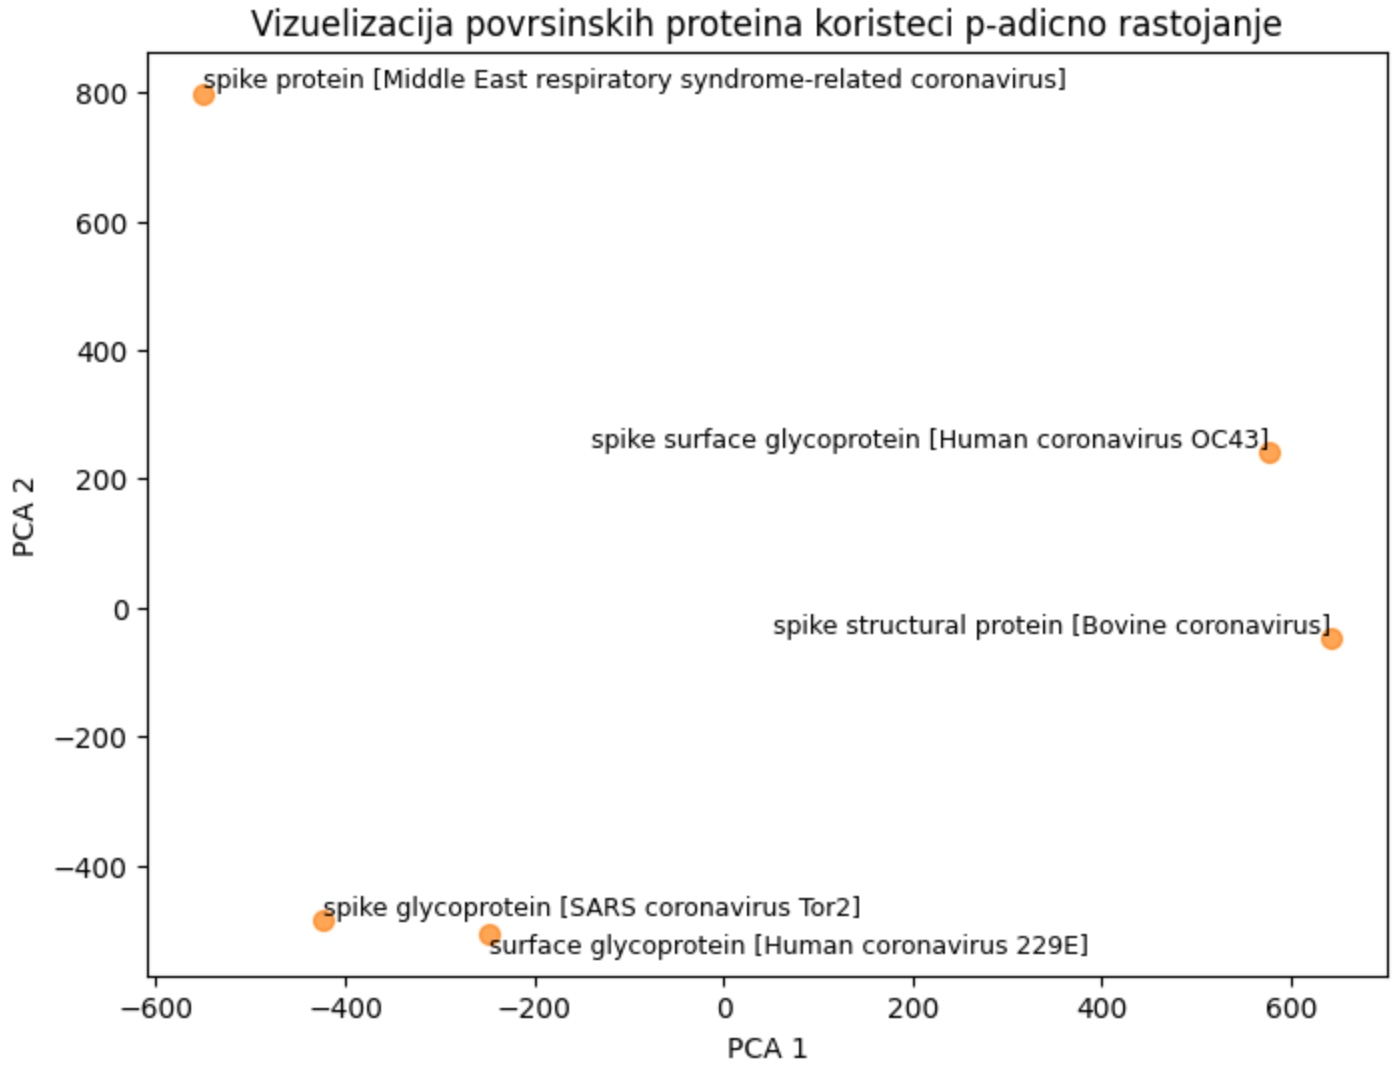
\includegraphics[width=1\textwidth]{slika27.jpeg}
  \caption{Vizuelizacija površinskih proteina koristeći p-adično rastojanje}
  \label{fig:my_label}
\end{figure}


\newpage
Analizirajući dobijene rezultate, primećujemo da iako su numeričke vrednosti udaljenosti značajno različite između ove dve metode, obrasci udaljenosti među površinskim proteinima su slični. 

\bigskip
Oba skupa rezultata pokazuju slične obrasce među određenim koronavirusima. Površinski proteini Human coronavirus 229E i SARS coronavirus Tor2, kao i Bovine coronavirus i Human coronavirus OC43, pokazuju tendenciju da budu međusobno bliži nego što su u odnosu na površinski protein iz Middle East respiratory syndrome-related coronavirus.

\bigskip
Izbor odgovarajuće metode zavisi od specifičnih zahteva istraživanja i potreba analize. Klasterovanje na osnovu edit rastojanja može pružiti korisne uvide u strukturu sličnosti kada je potrebno sagledati globalne genetske razlike. Sa druge strane, p-adična rastojanja su od velike važnosti kada je potrebno detaljno istražiti lokalne mutacije koje mogu imati značajan biološki uticaj, na primer, na funkciju proteina.



\newpage
\section{Zaključak}
U ovom seminarskom radu istraživali smo uticaj p-adičnog rastojanja na genetski kod koronavirusa i poredili dobijene rezultate sa rezultatma korišćenjem već tradicionalnih metoda u bioinformatici.

\bigskip
Hamingovo rastojanje na kodonima pruža brzu i relativno preciznu analizu proteina, dok klasterovanje na osnovu edit rastojanja omogućava sporiju, ali detaljniju analizu, fokusiranu na strukturne razlike.

\bigskip
Ključna prednost p-adičnih rastojanja je u tome što p-adična metrika pridaje najveći značaj razlici na prvom, a najmanji na poslednjem nukleotidu u kodonu, što je u skladu sa standardnim genetskim kodom. Zbog toga ova metoda omogućava dublje razumevanje veze između kodona i aminokiselina, što je od suštinskog značaja za proučavanje funkcionalnih karakteristika proteina. 


\bigskip
Na osnovu ovih nalaza, možemo zaključiti da p-adično rastojanje može postati ključan alat u bioinformatici zbog svoje sposobnosti da otkrije lokalne genetske razlike i pruži dublje razumevanje strukture genoma.




\newpage
\addcontentsline{toc}{section}{Reference}
\renewcommand{\refname}{Reference}
\begin{thebibliography}{9}
    \bibitem{cock2009biopython} Cock, P.J.A., et al. (2009). Biopython: freely available Python tools for computational molecular biology and bioinformatics. \textit{Bioinformatics}, 25(11), 1422-1423. \url{https://doi.org/10.1093/bioinformatics/btp163}.
    \bibitem{pedregosa2011scikit} Pedregosa, F., et al. (2011). Scikit-learn: Machine Learning in Python. \textit{Journal of Machine Learning Research}, 12, 2825-2830. \url{https://www.jmlr.org/papers/volume12/pedregosa11a/pedregosa11a.pdf}.
    \bibitem{harris2020array} Harris, C.R., et al. (2020). Array programming with NumPy. \textit{Nature}, 585, 357-362. \url{https://doi.org/10.1038/s41586-020-2649-2}.
    \bibitem{mckinney2010data} McKinney, W. (2010). Data Structures for Statistical Computing in Python. \textit{Proceedings of the 9th Python in Science Conference}, 51-56. \url{https://doi.org/10.25080/Majora-92bf1922-00a}.
    \bibitem{hunter2007matplotlib} Hunter, J.D. (2007). Matplotlib: A 2D Graphics Environment. \textit{Computing in Science \& Engineering}, 9(3), 90-95. \url{https://doi.org/10.1109/MCSE.2007.55}.
    \bibitem{waskom2020seaborn} Waskom, M., et al. (2020). seaborn: statistical data visualization. \textit{Journal of Open Source Software}, 6(60), 3021. \url{https://doi.org/10.21105/joss.03021}.
    \bibitem{github_link1} Jelisaveta Gavrilović. (2024). IP2-bioinformatics. \url{https://github.com/jelisavetagavrilovic/IP2-bioinformatics}.  
    \bibitem{github_link2} Marko Paunović. (2024). IP2-Bioinformatics. \url{https://github.com/MarkoPaunovic14/IP2-Bioinformatics}.
    \bibitem{bernfield1965} Bernfield, M.R., \& Nirenberg, M.W. (1965). RNA codewords and protein synthesis. \textit{Science}, 147(3657), 479-484. \url{https://doi.org/10.1126/science.147.3657.479}.
    \bibitem{ncbi_database} National Center for Biotechnology Information. (s.d.). Databases. \url{https://www.ncbi.nlm.nih.gov/genbank/}.
    \bibitem{dragovic2006} Dragovich, B., Dragovich, A., 2006. A p-adic model of DNA sequence and genetic code. \url{https://arxiv.org/abs/q-bio/0607018v1}

\end{thebibliography}


\end{document}


